\documentclass[a4paper,12pt]{memoir}
%%%%%%%%%%%%%%%%%%%%%%%%%%%%%%%%%%%%%%%%%%%%%%%%%%%%%%%%%%%%%%%%%%%%%%%%%%%%%
% EDIT HERE!!!
%%%%%%%%%%%%%%%%%%%%%%%%%%%%%%%%%%%%%%%%%%%%%%%%%%%%%%%%%%%%%%%%%%%%%%%%%%%%%
\def\candidate{First Last} % Your name
\def\thesistitle{A Very Very Long Title of the Super-Wonderful PhD Thesis Should Be Avoided If Possible} % Be as short as you can!! No more than 10 words
\def\keywords{Subject 1, Subject 2}
\def\advisor{Prof. First Last} 
\def\headphdprogram{Prof. First Last}
\def\refereeone{\textnormal{Prof. First Last}, \textit{institution}}
\def\refereetwo{\textnormal{Prof. First Last}, \textit{institution}}
\def\ciclo{XXXII}
% End EDIT
%%%%%%%%%%%%%%%%%%%%%%%%%%%%%%%%%%%%%%%%%%%%%%%%%%%%%%%%%%%%%%%%%%%%%%%%%%%%%

\usepackage[utf8]{inputenc}

\addtolength{\textwidth}{40pt}
\addtolength{\foremargin}{-40pt}
\addtolength{\spinemargin}{-40pt}
\setlrmarginsandblock{2.8cm}{2.8cm}{*}
\setulmarginsandblock{2.8cm}{*}{1}
\checkandfixthelayout%
\headsep=30pt
\linespread{1.1}

\usepackage[draft,inline,nomargin]{fixme}
\usepackage[round]{natbib}
\usepackage{graphicx}
\graphicspath{{./Figures/}}
\usepackage{xcolor}
\usepackage[pdftex]{hyperref}
\hypersetup{
  hidelinks,
  linkbordercolor=white,
  citebordercolor=white,
  urlbordercolor=white,
  filebordercolor=white}

\let\footruleskip\undefined %correct bug in footruleskip definition in
                            %memoir and fancyhdr
\usepackage{fancyhdr}
\pagestyle{fancy}
\renewcommand{\chaptermark}[1]{\markboth{#1}{}}
\renewcommand{\sectionmark}[1]{\markright{\thesection\ #1}}
\fancyhf{}
\fancyhead[LE,RO]{\fontfamily{phv}\selectfont\thepage}
\fancyhead[LO]{\rightmark}
\fancyhead[RE]{\fontfamily{phv}\selectfont\bfseries\leftmark}
\renewcommand{\headrulewidth}{0.1pt}
\renewcommand{\footrulewidth}{0pt}

\usepackage{verbatim}
\usepackage{url}
\usepackage{hyphenat}

\usepackage{amsmath,amsfonts,amssymb,amsthm}
\usepackage{latexsym}
\usepackage{array}
\usepackage{tocbibind}
\usepackage{listings}
\usepackage[retainorgcmds]{IEEEtrantools}

\usepackage{algorithmic}
\usepackage{algorithm2e}
\usepackage{color}
\usepackage{textcomp}
\usepackage{stackengine}

\hypersetup{ 
  pdfpagelayout=SinglePage, % default
  pdfpagemode=UseOutlines, % default
  bookmarksopen, % default
  bookmarksopenlevel=2, % default;
  pdftitle={\candidate's PhD thesis},
  pdfauthor={\candidate},
  pdfsubject={\thesistitle},
  pdfkeywords={PhD Program in Smart Computing, \keywords}
}

\usepackage[english]{babel}
\usepackage{blindtext}

\usepackage[sc]{mathpazo} % for maths
\usepackage{tgpagella} % as main font
\usepackage{nimbussans} % Helvetica

%\usepackage{makeidx}
%\makeindex

\usepackage{multirow}
\usepackage{acronym}
\usepackage{amsmath}
\usepackage{amssymb}
\usepackage{mathtools}
\usepackage{bm}
% \usepackage{subfigure}
\usepackage{subfig}
\usepackage{cleveref}
\usepackage{tikz}
\usetikzlibrary{positioning}
\usetikzlibrary{calc}


\definecolor{UFblue}{RGB}{12, 71, 123}



\newcommand{\svm}{\textbf{\emph{T-SVM}}}
\newcommand{\svmb}{\textbf{\emph{T2-SVM}}}
\newcommand{\lstmng}{\textbf{\emph{T2-2LSTM}}}
\newcommand{\lstmc}{\textbf{\emph{G-CLSTM}}}
\newcommand{\lstmb}{\textbf{\emph{G-2LSTM}}}

\newcommand{\site}{Main-site}
\newcommand{\fullSite}{Full-site}
\newcommand{\type}{Type}
\newcommand{\behaviour}{Behavior}

\newcommand{\matr}[1]{\bm{#1}}
\newcommand{\vect}[1]{\bm{#1}}
\newcommand{\dist}[1]{\mathcal{#1}}

\newtheorem{definition}{Definition}[section]

\def\RSet{\mathbb{R}}
\def\NSet{\mathbb{N}}
\def\XSet{\mathbb{X}}
\def\YSet{\mathbb{Y}}
\def\HSet{\mathbb{H}}
\def\prob{\mathbb{P}}
\def\expect{\mathbb{E}}
\def\define{\overset{\underset{\mathrm{def}}{}}{=}}

\DeclareMathOperator*{\argmax}{arg\,max}
\DeclareMathOperator*{\argmin}{arg\,min}

\def\MAX{MPM}
\def\loss{\mathcal{L}}

\def\maxi{MPMi}
\def\maxb{MPMb}


\acrodef{pac}[PAC]{Probably Approximately Correct}
\acrodef{iid}[i.i.d.]{indipendently and identically distributed}
\acrodef{ml}[ML]{Machine Learning}
\acrodef{ai}[AI]{Artificial Intelligence}
\acrodef{erm}[ERM]{Empirical Risk Minimization}
\acrodef{rtt}[RTT]{Registro Tumori della Toscana, Tumor Register of Tuscany}
\acrodef{icdo}[ICD-O]{International Classification of Diseases for Oncology}
\acrodef{icdo1}[ICD-O-1]{International Classification of Diseases for Oncology, first edition}
\acrodef{icdo3}[ICD-O-3]{International Classification of Diseases for Oncology, third edition}
\acrodef{hdr}[HDR]{Hospital Discharge Register}
\acrodef{cdf}[CDF]{Cumulative Distribution Function}
\acrodef{an}[AN]{Artificial Neuron}
\acrodef{ann}[ANN]{Artificial Neural Network}
\acrodef{cnn}[CNN]{Convolutional Neural Network}
\acrodef{rnn}[RNN]{Recurrent Neural Network}
\acrodef{mlp}[MLP]{Multilayer Perceptron}
\acrodef{lstm}[LSTM]{Long Short-Term Memory}
\acrodef{sgd}[SGD]{Stochastic Gradient Descend}
\acrodef{glove}[GloVe]{Global Vectors}
\acrodef{nb}[NB]{Naive Bayes}
\acrodef{svm}[SVM]{Support Vector Machine}
\acrodef{tfidf}[TF-IDF]{Term-Frequency Inverse-Document-Frequency}
\acrodef{map}[MAP]{Mean Average Precision}
\acrodef{relu}[ReLU]{Rectified Linear Unit}
\acrodef{max}[MPM]{Max Pooling Model}
\acrodef{gru}[GRU]{Gated Recurrent Unit}
\acrodef{nlp}[NLP]{Natural Language Processing}
\acrodef{bert}[BERT]{Bidirectional Encoder Representations from Transformers}
\acrodef{mlm}[MLM]{Masked Language Model}
\acrodef{nsp}[NSP]{Next Sentence Prediction}

\newcommand\floatwidth{0.45\textwidth}
\newcommand\attTableIcdoWidth{2.5cm}
\newcommand\attTableTextWidth{4.5cm}
\newlength\lunderset
\newlength\rulethick
\lunderset=1.7pt\relax
\rulethick=.8pt\relax
\def\stackalignment{l}
\newcommand\att[4][1]{\setbox0=\hbox{#2}%
  \stackunder[#1\lunderset-\rulethick]{\strut#2}{\color{#3!#4}\rule{\wd0}{\rulethick}}}

\definecolor{att}{rgb}{0, 1, 0}
\definecolor{attb}{rgb}{1, 0, 0}
\newcommand{\attvisB}[3]{\tikz[overlay]\node[fill=att!#2,inner sep=1pt, anchor=text, rectangle, rounded corners=1mm,draw=attb!#3] {#1};\phantom{#1}}

\makeatletter
  \providecommand*\setfloatlocations[2]{\@namedef{fps@#1}{#2}}
\makeatother
\setfloatlocations{figure}{htbp}
\setfloatlocations{table}{htbp}

\tikzstyle{every neuron}=[circle, draw, minimum size=1cm]
\tikzstyle{bias}=[circle,draw]
\tikzstyle{operation}=[circle,draw]
\tikzstyle{activation}=[draw]
\tikzstyle{layer}=[draw,minimum size=1cm]
\tikzstyle{delay}=[draw,minimum size=0.5cm,fill=black]
\tikzstyle{neuron missing}=[draw=none, scale=4,text height=0.333cm,execute at begin node=\color{black}$\vdots$]
\tikzstyle{vmissing}=[draw=none, scale=4,text height=0.333cm,execute at begin node=\color{black}$\vdots$]
\tikzstyle{hmissing}=[draw=none, scale=4,text width=0.41cm,execute at
begin node=\color{black}$\cdots$]
\tikzstyle{line}=[]
\tikzstyle{arrow}=[->, >=stealth]
\tikzstyle{arrowInverse}=[<-, >=stealth]
\tikzstyle{vectorLine}=[line width=0.6mm]
\tikzstyle{vectorArrow}=[->, >=stealth, line width=0.6mm]
\tikzstyle{border}=[draw]


\begin{document}
\hypersetup{pageanchor=false}
\thispagestyle{empty}
\pagenumbering{gobble}

{
  \fontfamily{phv}\selectfont

  \noindent
  \hspace*{-2.5cm}
\includegraphics[height=4cm]{firenze}
  \vskip 1.6ex

  \noindent
  \hspace*{1.3cm}{\large \textsc{PhD Program in Smart Computing}}

  \noindent
  \hspace*{1.3cm}{\textsc{Dipartimento di Ingegneria dell'Informazione (DINFO)}}

  \vfill
  \noindent
  \hspace*{1.3cm}
  \parbox{1.0\textwidth}{
    {\fontsize{30}{38}\selectfont \color{UFblue} \textbf{\nohyphens{\thesistitle}}\par}
    \vspace{6cm}
    \begin{flushright}
      \LARGE \textbf{\candidate}\\
      \vspace{8mm}
      \small Dissertation presented in partial fulfillment of the
      requirements\\
      for the degree of Doctor of Philosophy in Smart
      Computing
    \end{flushright}
  }
}

\newpage
\setulmarginsandblock{3.5cm}{3.5cm}{1}
{%
  \fontfamily{phv}
  \noindent
  \textit{PhD Program in Smart Computing}\\
  \textit{University of Florence, University of Pisa, University of Siena}

  \vfill
  \noindent
  % {\HUGE \textbf{\nohyphens{\thesistitle}}}
  {\fontsize{32}{38}\selectfont \textbf{\nohyphens{\thesistitle}}\par}
  \vfill
  \noindent
  {\Large \textbf{\candidate}}
}
\vfill
{
  % These are the required signatures according to unifi regulations
  \noindent
  \begin{minipage}{0.4\linewidth}
    \noindent
    {\fontfamily{phv}\textbf{Advisor:}}\\
    \vspace{7mm}
    \hrule
    \vspace{2mm}
    \advisor
  \end{minipage}

  \vspace{15mm}
  \noindent
  \begin{minipage}{0.4\linewidth}
    \noindent
    {\fontfamily{phv}\textbf{Head of the PhD Program:}}\\
    \vspace{7mm}
    \hrule
    \vspace{2mm}
    \headphdprogram
  \end{minipage}

  \vspace{15mm}

  % No signatures required here
  \noindent
  {\fontfamily{pag}\textbf{Evaluation Committee:}}\\
  \refereeone\\
  \refereetwo
}

\begin{center}
  \rule{\linewidth}{0.5mm}
  \fontfamily{pag}
  \ciclo\ ciclo --- October \number\the\year
  % \noindent Copyright~\copyright~\number\the\year~by \candidate.
\end{center}
\thispagestyle{empty}\null\vfil

\frontmatter
\newpage
\thispagestyle{empty}
%%%%%%%%%%%%%%%%%%%%%%%%%%%%%%%%%%%%%%%%%%%%%%%%%%%%%%%%%%%%%%%%%%%%%%%%%%%%% 
% EDIT HERE!!!
%%%%%%%%%%%%%%%%%%%%%%%%%%%%%%%%%%%%%%%%%%%%%%%%%%%%%%%%%%%%%%%%%%%%%%%%%%%%% 
\begin{flushright}
  \textit{To XXXXX} % Optional dedication
\end{flushright}
\null\vfil
% End EDIT
%%%%%%%%%%%%%%%%%%%%%%%%%%%%%%%%%%%%%%%%%%%%%%%%%%%%%%%%%%%%%%%%%%%%%%%%%%%%%
\newpage
\section*{Acknowledgments}
First of all, I would like to express my gratitude to my advisor
Prof. Paolo Frasconi for his expert guidance, for the important
insights he shared about the field of AI and the always new and
inspiring inputs about research.

Second, I would like to thank Leonardo Ventura, Prof. Gianni Amunni,
and ISPRO for giving me the opportunity to work with their data and
making this work of thesis possibile.

Thanks to Prof. S{\o}ren Brunak and Prof. Beatrice Lazzerini for
helping me advancing my 
research. 

I’m grateful to Prof. Enrico Vicario for introducing me to this
doctorate and to Prof. Simone Marinai for his precious advice.

A special thanks goes to the people who shared the AI-Team lab and the
Ph.D life with me. In alphabetical order: Daniele Baracchi, Samuele
Capobianco, Alessandro Lazzeri, Francesco Orsini, Giulia Pellegrini,
Dasara Shullani,
Alessandro Tibo, La Ode Toresano, Amin Zadenoori, and Zahra Ziran.

I would like to thank all my friends that were always there to support
me, root for me and cheer me up in moments of crisis and
doubt. Special mentions: Andrea Benassai, Vito Bonelli, Giulia
Bondielli, Giulia Bono, Tiberio Uricchio. Thanks to my dear family
Mauro, Rosa, and Simone for their presence and affection throughout my
whole life. Thanks to Fede for all the help that she gave me in this
thesis and in my whole life and for loving me dearly. Last but not
least, thanks to Spallina.


\newpage
\begin{abstract}
  \blindtext % Put your abstract here - don't exceed one page
\end{abstract}
\newpage

\pagenumbering{arabic}
\hypersetup{pageanchor=true}

\mainmatter
\tableofcontents
% \newpage\listoffigures% optional
% \newpage\listoftables% optional

%%%%%%%%%%%%%%%%%%%%%%%%%%%%%%%%%%%%%%%%%%%%%%%%%%%%%%%%%%%%%%%%%%%%%%%%%%%%%
% EDIT HERE!!!
%%%%%%%%%%%%%%%%%%%%%%%%%%%%%%%%%%%%%%%%%%%%%%%%%%%%%%%%%%%%%%%%%%%%%%%%%%%%%
\chapter{Introduction}
\label{ch:introduction}

\section{Cancer registries}
Cancer is a major concern worldwide, as it decreases the quality of
life and leads to premature mortality. In addition it is one of the
most complex and difficult-to-treat
diseases, with significant social implications, both in terms of
mortality rate and in terms of costs associated with treatment and
disability~\cite{sullivan_delivering_2011,b._stewart_world_2014,desantis_cancer_2014,siegel_cancer_2016}.
Measuring the burden of disease is one of the main concerns of public
healthcare operators. Suitable measures are necessary to describe the general state
of population’s health, to establish public health goals and to
compare the national health status and performance of health systems
across countries. Furthermore, such studies are needed to assess the
allocation of health care and health research resources across disease
categories and to evaluate the potential costs and benefits of public
health interventions~\cite{brown_burden_2001}.

Cancer registries emerged during the last few decades as a strategic
tool to quantify the impact of the disease and to provide analytic
data to healthcare operators and decision makers.  Cancer registries
use administrative and clinical data sources in order to identify all
the new cancer diagnoses in a specific area and time period and
collect incidence records that provide details on the diagnosis and
the outcome of treatments.  Mining cancer registry datasets can help
towards the development of global surveillance
programs~\cite{tourassi_deep_2017} and can provide important insights
such as survivability~\cite{delen_predicting_2005}.  Although data
analysis software would best operate on structured representations of
the reports, pathologists normally enter data items as free text in
the local country language. This requires intelligent algorithms for
medical document information extraction, retrieval, and
classification, an area that has received significant attention in the
last few years (see, e.g.,~\cite{mujtaba_clinical_2019} for a recent
account and \cite{yim_natural_2016} for the specific case of cancer).

\section{\ac{icdo}}\label{sec:icdoCodes}
Pathology reports can be classified according
to codes defined in the \ac{icdo3}
system~\cite{fritz_international_2000}, a specialization of the ICD
for the cancer domain which is internationally adopted as the standard
classification for topography and
morphology~\cite{airtum_handbook_2008}.  The development of text
analysis tools specifically devoted to the automatic classification of
incidence records according to ICD-O3 codes has been addressed in a
number of previous papers. However, these
works have either focused on reasonably large datasets but
using simple linear classifiers based on bag-of-words representations
of text~\cite{jouhet_automated_2011,kavuluru_automatic_2013}, or
applied recent state-of-the-art deep learning
techniques~\cite{gao_hierarchical_2018,qiu_deep_2018} but using
smaller datasets and restricted to a partial set of
tumors. Additionally, the use of deep learning techniques usually
requires accurate domain-specific word vectors (embeddings of words in
a vector space) that can be derived from word co-occurrences in large
corpora of unlabeled
text~\cite{mikolov_linguistic_2013,pennington_glove:_2014,devlin2018bert}. Large
medical corpora are easily available for English (e.g. PubMed) but not
 for other languages.

A topographical \ac{icdo3} code is structured as \emph{Cmm.s} where
\emph{mm} represent the main site and \emph{s} the subsite. For example, \emph{C50.2}
is the code for the upper-inner quadrant (\emph{2}) of breast (\emph{50}).

A morphological \ac{icdo3} code is structured as \emph{tttt/b}
where \emph{tttt} represent the cell type and \emph{b} the tumor
behavior (benign, uncertain, in-situ, malignant primary site,
malignant metastatic site). For example, \emph{8140/3}
is the code for an adenocarcinoma (\emph{adeno 8140};
\emph{carcinoma 3}).

\section{Existing works on \ac{icdo}}
Early works for ICD-O3 code assignment were structured on rule-based
systems, where the code was assigned by creating a set of handcrafted
text search queries and combining results by standard Boolean
operators~\cite{crocetti_automatic_2004}. In order to prevent spurious
matches, rules need to be very specific, making it very difficult to
achieve a sufficiently high recall on future (unseen) cases.

A number of studies reporting on the application of machine learning
to this problem have been published during the last decade. Direct
comparisons among these works are impossible due to the (not
surprising) lack of standard publicly available datasets and the
presence of 
heterogeneous details in the settings. Still, we highlight the main
differences among them in order to provide some 
background. In~\cite{jouhet_automated_2011}, the authors employed
support vector machine (SVM) and Naive Bayes classifiers on a small
dataset of $5\,121$ French pathology reports and a reduced number of
target classes (26 topographic classes and 18 morphological classes),
reporting an accuracy of 72.6\% on topography and 86.4\% on morphology
with SVM. A much larger dataset of $56\,426$ English reports from the
Kentucky Cancer Registry was later employed
in~\cite{kavuluru_automatic_2013}, where linear classifiers (SVM,
Naive Bayes, and logistic regression) were also compared but only on
the topography task and using 14, 42, and 57 classes. The authors
reported a micro-averaged F1 measure of 90\% when using SVM with both
unigrams and bigrams. Still, the bag-of-words representations used by
these linear classifiers do not consider word order and are
unable to capture similarities and relations among words (which are
all represented by orthogonal vectors). Deep learning techniques are
known to overcome these limitations but were not applied to this
problem until very recently. In~\cite{qiu_deep_2018}, a \ac{cnn}
architecture fed by word vectors pretrained on 
PubMed was applied to a small corpus of 942 breast and lung cancer
reports in English with 12 topography classes; the authors demonstrate
the superiority of this approach compared to linear classifiers with
significant increases in both micro and macro F1
measures. In~\cite{gao_hierarchical_2018}, the same research group also
experimented on the same dataset using \acp{rnn}
with hierarchical attention~\cite{yang_hierarchical_2016}, obtaining
further improvements over the CNN architecture.

\section{Motivation and contributions}\label{sec:motivation}
With this work we want to answer to some questions.
\begin{description}
\item[Q1] At the best of our
  knowledge, there are no large scale studies on deep learning method
  applied to pathology reports. Cancer registries collect large amount of
  records and invest time labeling them with topographical and
  morphological codes. Existing works focus on \ac{icdo} classification
  of small datasets or using few 
  classes. We want to make a step further applying deep learning
  techniques to a large scale dataset.
\item[Q2] We want to apply novel deep learning techniques, like
  attention models and \ac{bert}, to cancer pathology reports text
  classification. We want to propose
  experiments to assess how they perform on this kind of data.
\item[Q3] It is not yet clear from the literature if, in this domain,
  bag-of-words techniques are inferior to deep learning
  techniques. The structure of the sentences in italian-language 
  cancer pathology reports differs substantially from the structure of the text
  where \ac{rnn} methods are usually employed. The records often
  do not present the usual subject-verb-object structure.
\item[Q4] It is not clear if the use of novel attention-based and
  hierarchical techniques 
  represents an improvement with respect to simpler \ac{rnn} methods on this
  kind of text. 
\item[Q5] It is not clear the contribution and the applicability of
  unsupervised learning techniques to uncommon text corpora. Usually,
  word vectors are trained on long english text corpora, taken from
  Wikipedia, Gigaword, or similar. Our documents not only are in a
  different language, but they also have a different structure.
\item[Q6] We want to evaluate the possibility to give
  some interpretation to the notoriously uninterpretable deep learning
  models. 
\end{description}


%%% Local Variables:
%%% mode: latex
%%% TeX-master: "thesis"
%%% End:

\chapter{Background}
\label{ch:background}


%%% Local Variables:
%%% mode: latex
%%% TeX-master: "thesis"
%%% End:

\chapter{\ac{icdo} classification improved}
\label{ch:icdo}

\section{Dataset}
For the experiments in this chapter, we further refined the dataset
explained in \cref{sec:dataset}. We removed duplicate
reports and reports labeled with extremely rare (1048
samples that not
appear in either training, validation, and test sets) ICD-O3 codes. We
obtained in the end 
a dataset suitable for supervised learning consisting of $85\,170$
labeled records over $203$ morphological classes and $68$
topological classes (see below).

\section{Prediction tasks}
We defined two multi-class classification tasks: (1) main tumor site
prediction ($68$ mutually exclusive classes) and (2) morphology
prediction ($203$ mutually exclusive
classes). Although the two tasks maybe somewhat correlated, we did not
attempt multi-task approaches given the small number of tasks and
large enough size of the dataset.

As in \cref{ch:icdoFirst}, the dataset is highly unbalanced.

\subsection{Plain model}
\label{sec:model}
In our setting, a dataset $\mathcal{D}=\{(\vect{x}^{(i)},y^{(i)})\}$
consists of variable length sequence vectors $\vect{x}^{(i)}$, where
$x^{(i)}_t$, for $t=1,\dots,T^{(i)}$ is the $t$-th word in the $i$-th
document, and associated target classes
$y^{(i)}\in\{1,\dots,K\}$. Unless necessary, we will drop the
superscript in the following to keep notation simple.  Sequences will
be denoted in boldface. The RNN-based sequence classifiers used in
this work compute their predictions $f(\vect{x})$ as follows:
\begin{align}
  e_t &=& E(x_t;\theta^e),\label{eq:embed}\\
  h^f_t &=& F(e_t,h^f_{t-1};\theta^f),\label{eq:maxModelRL}\\  
  h^r_t &=& R(e_t,h^r_{t+1};\theta^r),\label{eq:maxModelRR}\\
  u_t &=& G(h_t;\theta^h),\label{eq:maxModelF}\\
  \phi & =& A(\vect{h},\vect{u};\theta^a),\label{eq:aggregation}\\
  f(\vect{x}) &=& g(\phi;\theta^c).\label{eq:maxModelC}
\end{align}
$E$ is an embedding function mapping words into $p$-dimensional real
vectors (where embedding parameters $\theta_e$ can be either
pretrained and adjustable or fixed, see Section~\ref{sec:word-vectors}
below.  Functions $F$ and $R$ corresponds to (forward and reverse)
dynamics that can be described in term of several (possibly layered)
recurrent cells. In this work we focus on \ac{gru}
cells~\cite{cho2014properties} for their simplicity and because
preliminary experiments revealed no advantages over long-short term
memory cells~\cite{hochreiter1997long} on our data. Each vector $h_t$,
the concatenation of $h^f_t$ and $h^r_t$, can be interpreted as latent
representations of the information contained at position $t$ in the
document. $G$ is an additional \ac{mlp} mapping each latent vector into a
vector $u_t$ that can be seen as contextualized representation of the
word at position $t$. $A$ is an aggregation function that creates a
single $d$-dimensional representation vector for the entire sequence
and $g$ is a softmax layer. Possible choices for the aggregator
function include:
\begin{itemize}
\item $\phi=(h^f_T,h^r_1)$, which just
  extract the extreme latent representations; these may be in
  principle sufficient since they depend on the whole sequence due to
  bidirectional dynamics; note however that this approach may require
  long-term dependencies to be effectively learned.
\item
  % $\phi = \sum_t a_t(\vect{u};\theta^a) h_t$,
  $\phi = \sum_t a_t(\vect{u};\theta^a) u_t$,
  using an attention mechanism as in~\cite{yang_hierarchical_2016}; in
  this case, (scalar) attention weights are computed as
  \begin{align*}
    c_t&=&C(\vect{u};\theta^a),\\
    a_t(\vect{u};\theta^a) &=& \frac{e^{\langle c, c_t\rangle}}
    {\sum_i{e^{\langle c, c_i\rangle}}},\\
  \end{align*}
  %$$
  %a_t(\vect{u};\theta^a) = \frac{e^{\langle \theta^a, u_t\rangle}}
  %{\sum_s{e^{\langle \theta^a, u_s\rangle}}}
  %$$
  where $C$ is a single layer that map the representation $u_t$ of the
  word to a hidden representation $c_t$, then the importance of the word is
  measured as a similarity with a context vector $c$ that is learned
  with the model and can be seen as an embedded representation of an
  high level query as in memory networks \cite{sukhbaatar2015end}.
\item $\phi = \max_t u_t$ where the maximum is taken element-wise
  along the sequence; this approach can be interpreted either as a
  simplified (parameter-less) attention mechanism or a bag-layer as
  proposed in the context of multi-instance
  learning~\cite{tibo2017network}; in this case each ``feature''
  $\phi_j$ will be positive if at least one of $u_{j,1},\dots,u_{j,T}$
  is positive; the resulting classifier will find it easy to create
  decision rules predicting a document as belonging to a certain class
  if a given set of contextualized word representations are present
  and another given set of contextualized word representations are
  absent in the sequence.
\end{itemize}

The parameters $\theta^f,\theta^r,\theta^h$ and $\theta^a$ (if
present) are determined by minimizing a loss function $\loss$
(categorical cross-entropy in our case) on training data:
\begin{equation}
  \hat \theta = \mathrm{arg}\min_\theta\sum_{(\vect{x},y)\in\mathcal{D}}\loss\left(y,f(\vect{x})\right).
\end{equation}

% $e:\XSet\rightarrow\RSet^k$ is an embedding function that transforms
% sequence elements in tensors $\vect{x}_{i,j}=e(x_{i,j})$ of
% dimension $k$ that can be parsed by the
% model. $g:\YSet\rightarrow[0,1]^q$ is an embedding function that
% transforms sequences labels in one-hot encodings of a coherent
% dimension $q$.
\subsection{Hierarchical model}
\label{sec:modelh}
We compared the model of \cref{sec:model} with a hierarchical setting,
similarly to other works \cite{yang_hierarchical_2016}. In this
setting our dataset $\mathcal{D}=\{\vect{x}^{(i)},y^{(i)}\}$
consists of variable length sequence of sequence vectors
$\vect{x}^{(i)}$, where $x_{s,t}^{(i)}$, for $s=1,\dots,S^{(i)}$ and
$t=1,\dots,T^{(i,s)}$ is the $t$-th word of the $s$-th sentence in the
$i$-th document, and associated target classes
$y^{(i)}\in\{1,\dots,K\}$. The prediction $f(\vect{x})$ is calculated:
\begin{align}
  e_{s,t} &=& E(x_{s,t};\theta^e),\label{eq:embedH}\\
  h^f_{s,t} &=& F(e_{s,t},h^f_{s,t-1};\theta^{f}),\label{eq:maxModelRLH}\\  
  h^r_{s,t} &=& R(e_{s,t},h^r_{s,t+1};\theta^{r}),\label{eq:maxModelRRH}\\
  u_{s,t} &=& G(h_{s,t};\theta^{h}),\label{eq:maxModelFH}\\
  \phi_s & =& A(\vect{h}_s,\vect{u}_s;\theta^{a}),\label{eq:aggregationH}\\
  w^f_{s} &=& F(\phi_{s},w^f_{s-1};\theta^{fs}),\label{eq:maxModelRLHS}\\  
  w^r_{s} &=& R(\phi_{s},w^r_{s+1};\theta^{rs}),\label{eq:maxModelRRHS}\\
  \psi & =& A(\vect{s},\vect{w};\theta^{a}),\label{eq:aggregationHS}\\
  f(\vect{x}) &=& g(\psi;\theta^c).\label{eq:maxModelCH}
\end{align}
As in \cref{sec:model}, $E$ is an embedding function, $F$ and $R$
corresponds to forward and reverse dynamics,
$h_{s,t}=h_{s,t}^f\oplus h_{s,t}^r$ is the latent representation of
the information contained at position $t$ of the $s$-th sentence,
$u_{s,t}$ is the contextualized representation of the word at position
$t$ of the $s$-th sentence, and $A$ is an aggregation function that
creates a single representation for the entire sequence (of words in a
sentence for \eqref{eq:aggregationH}, of sentences in a document for
\eqref{eq:aggregationHS}). Furthermore, $w_s=w_s^f\oplus w_s^r$
can be interpreted as the
latent representation of the information contained in the sentence $s$
for the document

\section{Baseline}

\subsubsection{Linear classifiers}
The classic approach is to employ bag-of-words
representations of textual documents.
%In this approach, a document is 
%described by a \textit{set} or a \textit{multiset} of words.
%Multisets allow one to take into account the number of occurrences of
%a word in the document.
Vector representations of documents are easily
derived from bags-of-words either by using indicator vectors or taking
into account the number of occurrences of each word using the
\ac{tfidf}\cite{manning_introduction_2008}. In those representations,
frequent and non-specific terms receive a lower weight.

Bag-of-words representations (including those employing bigrams or
trigrams) enable the application of very simple text classifiers such
as \ac{nb} or \ac{svm} \cite{cortes-support-1995}, but they
suffer two fundamental problems. First, the relative order of terms in
the documents is lost, making it impossible to take advantage of the
syntactic structure of the sentences. Second, distinct words have an
orthogonal representation even when they are semantically
close. As detailed in the next section, word vectors can be used to
address the second limitation and also allow us to take advantage of
unlabeled data, which can be typically be obtained in large amounts
and with little cost.

\subsubsection{\acs{bert}}
\ac{bert} \cite{devlin2018bert} is a recent model that represents the
state of the art in many \ac{nlp} related tasks
\cite{chatterjee2019semeval,hu2019introductory,lee2019biobert,tshitoyan2019unsupervised}.
It is a
bi-directional pre-training model backboned by the Transformer Encoder
\cite{vaswani2017attention}. It is an attention-based technique that
learns context-dependent word representation on large unlabeled
corpora, and then the model is fine tuned end to end on specific labeled
tasks. During pre-training, the model is trained
on unlabeled data over two different tasks. In \ac{mlm} some tokens
are masked and the model is trained to predict those token based on
the context. In \ac{nsp} the model is trained to understand the
relationship between sentences predicting if two sentences are actually
consecutive or if they where randomly replaced (with 50\%
probability). After the pre-training, the model is fine-tuned to the
specific task.


\subsection{Hyperparameters}
The hyperparameters defined in \eqref{eq:embed}~-~\eqref{eq:maxModelC}
and \eqref{eq:embedH}~-~\eqref{eq:maxModelCH} control the structure of
the model. $\theta^e$ refers to \ac{glove}
hyperparameters~\cite{pennington_glove:_2014}, we found with an
intrinsic evaluation the better configuration was $60$ for the vector
size, $15$ for the window size, and $50$ iterations. $\theta^f$,
$\theta^r$, $\theta^{fs}$, and $\theta^{rs}$ set the number of
\ac{gru} layers ($\theta_{(l)}$) and the number of unit per each layer
($\theta_{(d)}$). 
layer. $G$ is a \ac{mlp}, thus $\theta^h$ controls the number of
layers and the dimension. To limit the
hyperparameters space, we decided to
make equal-dimension stacked layers in case of more than one,
regarding $F$, $R$, and $G$. $\theta^a$ controls the
kind of aggregating function of $A$, and in case of \emph{attention}
it controls the dimension of the attention layer. Finally $\theta^c$ controls the
data-dependent output dimension.

In our experiments we defined five different settings that we named
with acronyms. In \ac{max} we used the \emph{max} aggregation function
in the plain model of \cref{sec:modelh}. We determined the
hyperparameters evaluating the validation set in the space (with the
better configuration underlined):
\begin{align*}
  \theta_{(l)}^f=\theta_{(l)}^r&\in&[\underline{1},2],\\
  \theta_{(d)}^f=\theta_{(d)}^r&\in&[2,4,8,16,32,64,\underline{128},256,512],\\
  \theta_{(l)}^h&\in&[\underline{1},2,4],\\
  \theta_{(d)}^h&\in&[2,4,8,16,32,64,128,256,\underline{512},1024,2048],
\end{align*}
for the \emph{main site} task, and:
\begin{align*}
  \theta_{(l)}^f=\theta_{(l)}^r&\in&[\underline{1}],\\
  \theta_{(d)}^f=\theta_{(d)}^r&\in&[2,4,8,16,32,64,\underline{128},256,512],\\
  \theta_{(l)}^h&\in&[\underline{1},2,4],\\
  \theta_{(d)}^h&\in&[2,4,8,16,32,64,\underline{128},256,512,1024,2048],
\end{align*}
for the \emph{morphology} task.

In \ac{softmax} we used the \emph{attention} aggregation function in the
plain model. The hyperparameters
space was:
\begin{align*}
  \theta_{(l)}^f=\theta_{(l)}^r&\in&[\underline{1}],\\
  \theta_{(d)}^f=\theta_{(d)}^r&\in&[64,\underline{128},256],\\
  \theta_{(l)}^h&\in&[0,\underline{1}],\\
  \theta_{(d)}^h&\in&[256,\underline{512},1024],\\
  \theta_{(d)}^a&\in&[128,\underline{256},512,1024],
\end{align*}
for the site, and:
\begin{align*}
  \theta_{(l)}^f=\theta_{(l)}^r&\in&[\underline{1}],\\
  \theta_{(d)}^f=\theta_{(d)}^r&\in&[64,128,\underline{256}],\\
  \theta_{(l)}^h&\in&[0,\underline{1}],\\
  \theta_{(d)}^h&\in&[64,\underline{128},256],\\
  \theta_{(d)}^a&\in&[128,\underline{256},512,1024],
\end{align*}
for the morphology.

In \ac{maxh} we used the \emph{max} aggregation in the hierarchical
model of \cref{sec:modelh}. The hyperparameters space was:
\begin{align*}
  \theta_{(l)}^f=\theta_{(l)}^r=\theta_{(l)}^{fs}=\theta_{(l)}^{rs}&\in&[\underline{1}],\\
  \theta_{(d)}^f=\theta_{(d)}^r=\theta_{(d)}^{fs}=\theta_{(d)}^{rs}&\in&[32,\underline{64},128,256],\\
  \theta_{(l)}^h&\in&[0,1,\underline{2},4],\\
  \theta_{(d)}^h&\in&[256,512,\underline{1024},2048],\\
\end{align*}
for the site, and:
\begin{align*}
  \theta_{(l)}^f=\theta_{(l)}^r=\theta_{(l)}^{fs}=\theta_{(l)}^{rs}&\in&[\underline{1}],\\
  \theta_{(d)}^f=\theta_{(d)}^r=\theta_{(d)}^{fs}=\theta_{(d)}^{rs}&\in&[32,\underline{64},128,256],\\
  \theta_{(l)}^h&\in&[0,\underline{1},2,4],\\
  \theta_{(d)}^h&\in&[256,512,\underline{1024},2048],\\
\end{align*}
for the morphology.

In \ac{softmaxh} we used the \emph{attention} aggregation in the
hierarchical model. The hyperparameters space was:
\begin{align*}
  \theta_{(l)}^f=\theta_{(l)}^r=\theta_{(l)}^{fs}=\theta_{(l)}^{rs}&\in&[\underline{1}],\\
  \theta_{(d)}^f=\theta_{(d)}^r=\theta_{(d)}^{fs}=\theta_{(d)}^{rs}&\in&[32,64,\underline{128},256],\\
  \theta_{(l)}^h&\in&[0,\underline{1},2,4],\\
  \theta_{(d)}^h&\in&[256,512,\underline{1024},2048],\\
  \theta_{(d)}^a&\in&[64,\underline{128},256,512],
\end{align*}
for the site, and:
\begin{align*}
  \theta_{(l)}^f=\theta_{(l)}^r=\theta_{(l)}^{fs}=\theta_{(l)}^{rs}&\in&[\underline{1}],\\
  \theta_{(d)}^f=\theta_{(d)}^r=\theta_{(d)}^{fs}=\theta_{(d)}^{rs}&\in&[32,\underline{64},128,256],\\
  \theta_{(l)}^h&\in&[0,\underline{1},2,4],\\
  \theta_{(d)}^h&\in&[256,512,\underline{1024},2048],\\
  \theta_{(d)}^a&\in&[64,\underline{128},256,512],
\end{align*}
for the morphology.

In \ac{maxi} we used the \emph{max} aggregation in the plain
model. Also we set the model to be interpretable (see
\cref{sec:interpretability}). The hyperparameters space was:
\begin{align*}
  \theta_{(l)}^f=\theta_{(l)}^r&\in&[1,\underline{2},4],\\
  \theta_{(d)}^f=\theta_{(d)}^r&\in&[2,4,8,16,32,64,\underline{128},256,512],\\
  \theta_{(l)}^h&\in&[\underline{1},2,4],\\
  \theta_{(d)}^h&\in&[2,4,8,16,32,64,128,256,512,1024,2048],
\end{align*}
for the site, and:
\begin{align*}
  \theta_{(l)}^f=\theta_{(l)}^r&\in&[1,\underline{2},4],\\
  \theta_{(d)}^f=\theta_{(d)}^r&\in&[64,128,\underline{256},512],\\
  \theta_{(l)}^h&\in&[\underline{1}],\\
  \theta_{(d)}^h&\in&[],
\end{align*}
for the morphology. Note that in this setting the dimension of the
last layer of $G$ must be equal to the output dimension of the model
(and the softmax is applied directly after the aggregation $A$,
without any layer). Thus, $\theta_{(d)}^h$ refers only to the
layers before the last one, if they exists.




% The hyperparameters $\xi=\xi^l\cup\xi^r\cup\xi^h\cup\xi^c$ define the
% structure of the model. Regarding $\xi^l=\xi^r$ they define the type
% of \ac{rnn} that in our experiments can be \ac{lstm} or \ac{gru}, the
% number of stacked \ac{rnn} layers and the dimension of each
% layer. $\xi^h$ defines the number of layers in the first
% \ac{mlp} and their
% dimensions, moreover it defines the type of aggregating function $f$
% that in our experiments can be one of
% \begin{align}
%   f(\vect{a},\vect{b}) &= \left[\max(a_1,b_1),\dots,\max(a_l,b_l)\right];\\
%   f(\vect{a},\vect{b}) &= \left[\frac{a_1+b_1}{2},\dots,\frac{a_l+b_l}{2}\right];\\
%   f(\vect{a},\vect{b}) &= \left[a_1,\dots,a_l,b_1,\dots,b_l\right].\label{eq:aggregation}
% \end{align}
% $\xi^c$ defines the number of layers and their dimensions of the
% final classifier. The number of layers defined in $\xi^h$ can be
% equal to $0$. In such case, $\vect{h}_{i,j}$ is calculated:
% \begin{equation*}
%   \vect{h}_{i,j} = f(\vect{h}^l_{i,j},\vect{h}^r_{i,j}).
% \end{equation*}
% Also the number of layers defined in $\xi^c$ can be equal to $0$. In
% such case $\vect{\hat{y}}_i$ is calculated:
% \begin{equation*}
%   \vect{\hat y}_i = \max_j(\vect{h}_{i,j}).
% \end{equation*}


\section{Results}
\subsection{Artificial dataset}\label{sec:experiments}
Classic \ac{rnn} approaches exhibit some limits related to
memory. We designed an artificial experiment in
order to investigate how \ac{rnn} and \ac{max} address those
problems. The dataset 
$\mathcal{D}=(\vect{X}\in [0,\dots,9]^{n\times m},\vect{y}\in [0,1]^n)$ is
composed of $n$ sequences of length
$m$ of digits $x_{i,j}\in[0,\dots,9]$. If the $i$-th sequence contains
at least three consecutive digits
$x_{i,j-1},x_{i,j},x_{i,j+1}$ that concatenated represents a prime
number then the
sample is positive and labeled with $y_i=1$, otherwise is negative and
$y_i=0$.

We realized a series
$\mathcal{D}^{(m)}=(\vect{X}^{(m)},\vect{y}^{(m)})$ of balanced
datasets of increasing complexity. Each $\mathcal{D}^{(m)}$ has $100\ 000$
samples with 
sequence lengths of $m\in
[100,200,300,400,500,600,700,800,900,1000]$. We trained two models on
all the datasets: a plain \ac{gru} with hidden dimension $32$ and a
our model with max aggregation with same hidden dimension $32$. 

\begin{figure}
  \centering
  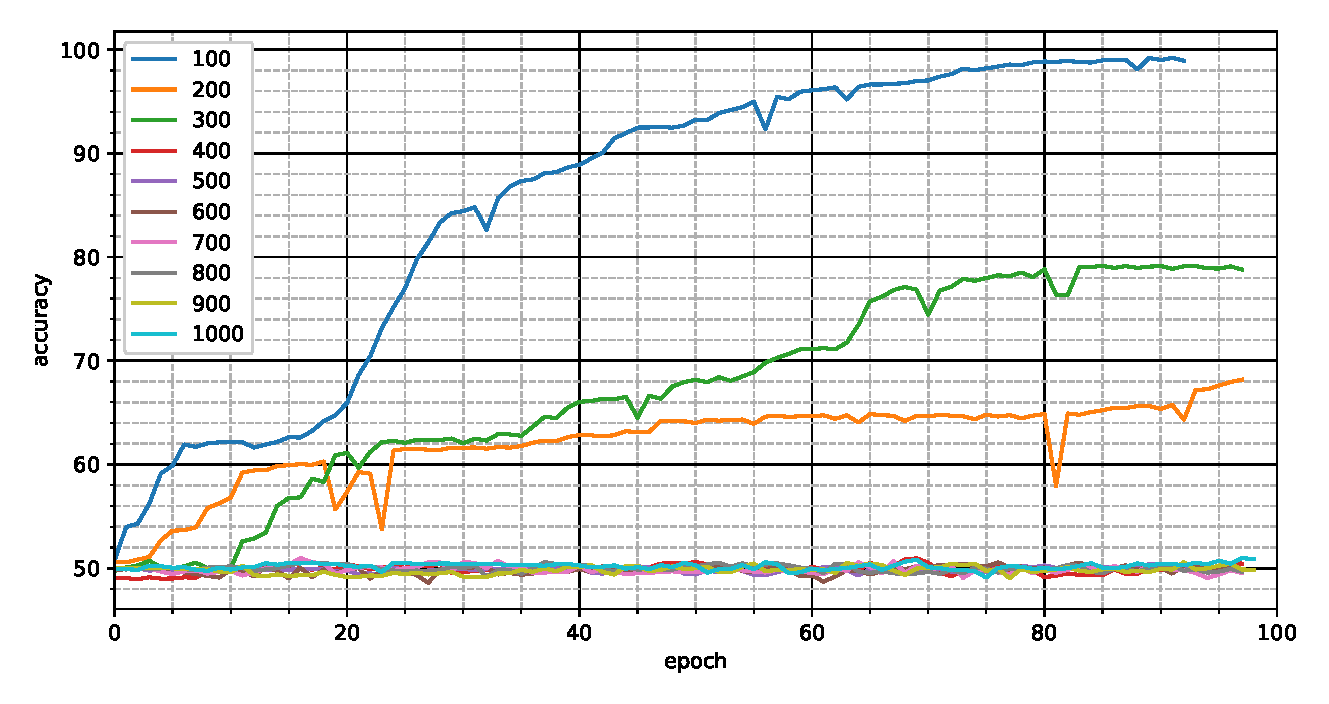
\includegraphics[width=\floatwidth]{imgMax/accuracy-base.eps}
  \caption{Accuracy of plain \ac{gru} on $\mathcal{D}^{(m)}$ for different dimensions of $m$.}
  \label{fig:testAccBase}
\end{figure}

\begin{figure}
  \centering
  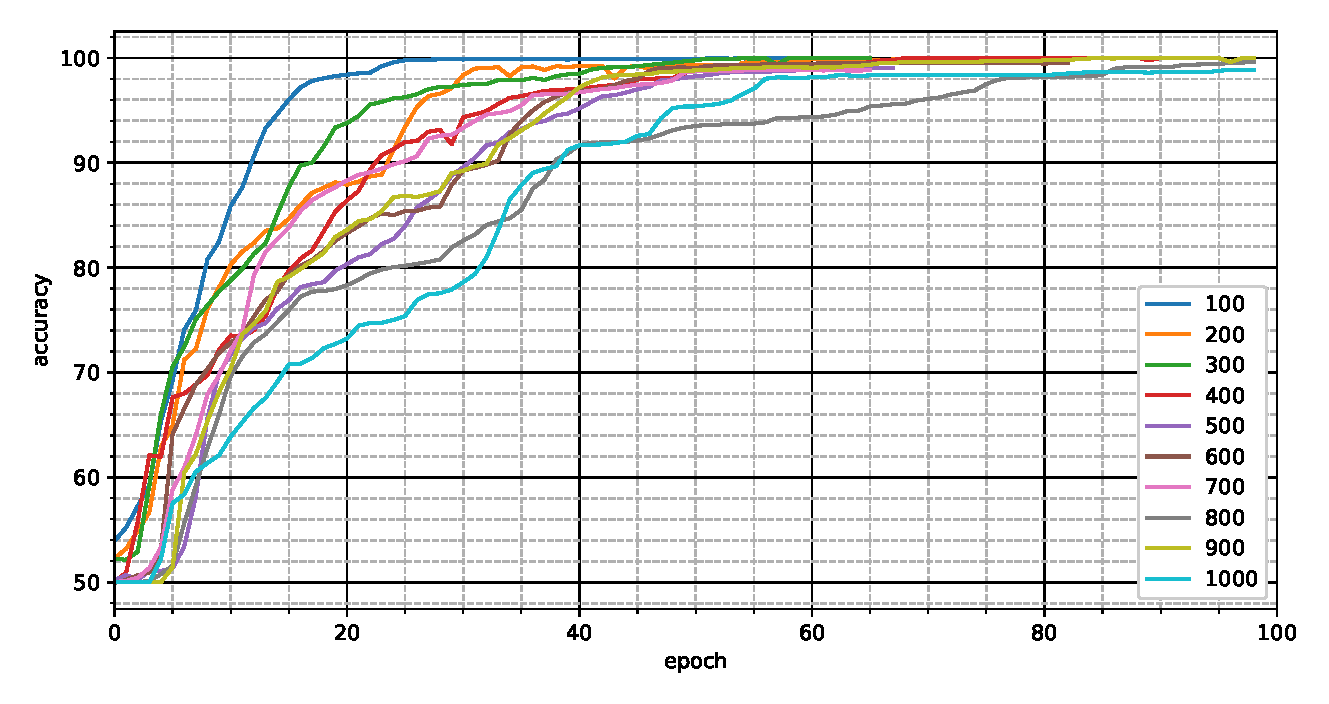
\includegraphics[width=\floatwidth]{imgMax/accuracy-max.eps}
  \caption{Accuracy of our model with max aggregation on $\mathcal{D}^{(m)}$ for different dimensions of $m$.}
  \label{fig:testAccMax}
\end{figure}

In \cref{fig:testAccBase} and \cref{fig:testAccMax} we compare
the learning curves of the base model with the ours. We can conclude
that our model degrades less than the baseline under the assumption of
having the same number of parameters.

\subsection{Interpretability}
\label{sec:interpretability}
The model is flexible enough to gain interpretability under certain
assumptions. If we remove the last layer in \eqref{eq:maxModelC},
the dimension of last layer in \eqref{eq:maxModelF}
needs to be equal to the
output dimension ($1$ for the artificial dataset, $68$ for the site
task, and $203$ for the 
morphology).
We hypothesize that in this case, the values of
$u_t$ (or the weighted values $a_t(\vect{u};\sigma^a)u_t$ if we use the
attention as aggregator) collect information on the importance of the
area 
around $x_t$ for the purpose of classification task. This
information can be
used to interpret the model decision. To validate the
hypothesis we performed the same experiment of \cref{sec:experiments}
with an interpretable model with a comparable number of parameters.

\begin{figure}
  \centering
  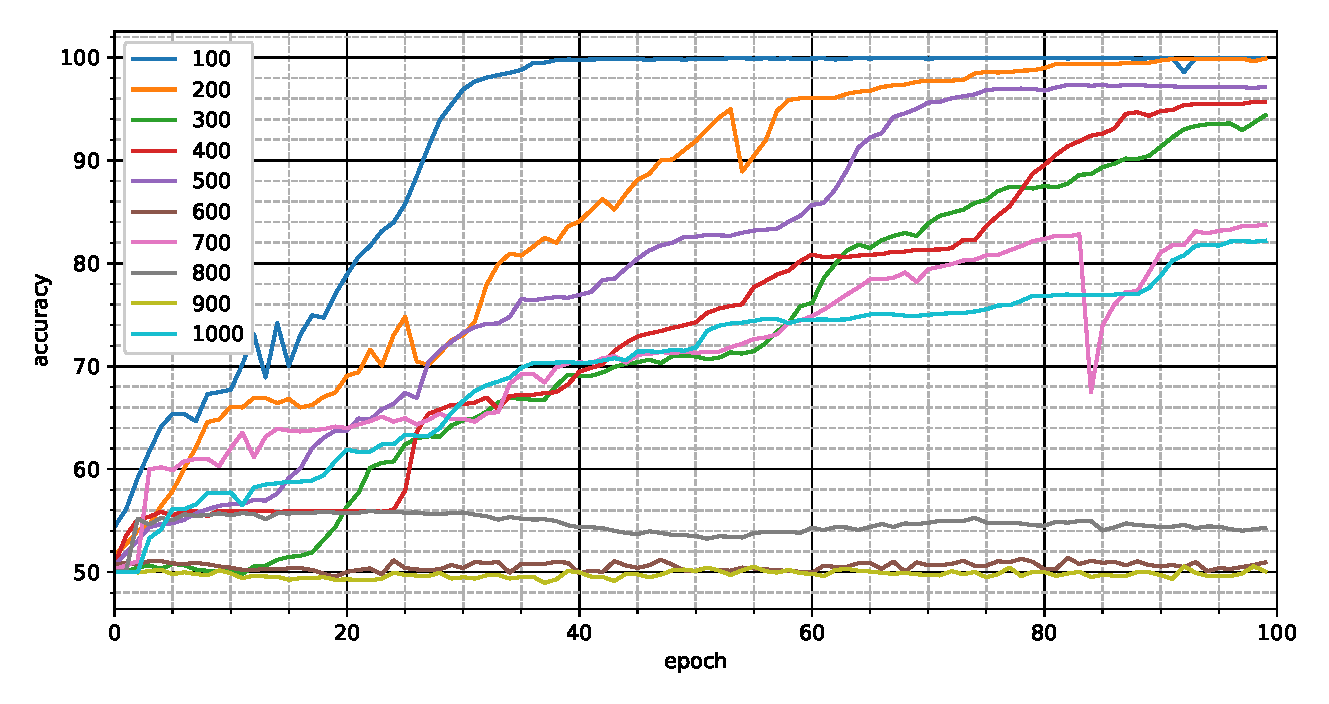
\includegraphics[width=\floatwidth]{imgMax/accuracy-int.eps}
  \caption{Accuracy of interpretable model with max aggregation on $\mathcal{D}^{(m)}$ for different dimensions of $m$.}
  \label{fig:testAccInt}
\end{figure}

\begin{figure}
  \centering
  \footnotesize
  \begin{tabular}{|p{\floatwidth}|}
    \hline
    \attvisB{0}{5}{0} \attvisB{9}{6}{0} \attvisB{2}{7}{0} \attvisB{1}{7}{0} \attvisB{8}{5}{0} \attvisB{4}{5}{0} \attvisB{2}{5}{0} \attvisB{8}{5}{0} \attvisB{9}{6}{0} \attvisB{1}{6}{0} \attvisB{4}{5}{0} \attvisB{6}{5}{0} \attvisB{8}{6}{0} \attvisB{8}{5}{0} \attvisB{6}{4}{0} \attvisB{6}{5}{0} \attvisB{8}{6}{0} \attvisB{7}{7}{0} \attvisB{3}{5}{0} \attvisB{0}{5}{0} \attvisB{2}{5}{0} \attvisB{5}{5}{0} \attvisB{9}{7}{0} \attvisB{7}{7}{0} \attvisB{9}{6}{0} \attvisB{5}{5}{0} \attvisB{8}{5}{0} \attvisB{2}{5}{0} \attvisB{4}{6}{0} \attvisB{9}{6}{0} \attvisB{5}{5}{0} \attvisB{5}{5}{0} \attvisB{6}{5}{0} \attvisB{5}{6}{0} \attvisB{1}{7}{0} \attvisB{7}{7}{0} \attvisB{6}{5}{0} \attvisB{3}{5}{0} \attvisB{2}{6}{0} \attvisB{2}{5}{0} \attvisB{2}{7}{0} \attvisB{1}{6}{100} \attvisB{3}{5}{100} \attvisB{1}{100}{100} \attvisB{2}{5}{0} \attvisB{5}{5}{0} \attvisB{0}{5}{0} \attvisB{8}{5}{0} \attvisB{9}{6}{0} \attvisB{5}{5}{0} \attvisB{4}{6}{0} \attvisB{0}{5}{0} \attvisB{3}{5}{0} \attvisB{2}{5}{0} \attvisB{3}{5}{0} \attvisB{0}{5}{0} \attvisB{6}{4}{0} \attvisB{0}{5}{0} \attvisB{0}{5}{0} \attvisB{8}{5}{0} \attvisB{6}{5}{0} \attvisB{7}{7}{0} \attvisB{9}{7}{0} \attvisB{1}{6}{0} \attvisB{6}{5}{0} \attvisB{4}{6}{0} \attvisB{0}{5}{0} \attvisB{5}{5}{0} \attvisB{7}{7}{0} \attvisB{0}{5}{0} \attvisB{6}{4}{0} \attvisB{4}{6}{0} \attvisB{6}{5}{0} \attvisB{0}{6}{0} \attvisB{6}{5}{0} \attvisB{1}{6}{0} \attvisB{5}{4}{0} \attvisB{4}{6}{0} \attvisB{3}{5}{0} \attvisB{2}{6}{0} \attvisB{5}{5}{0} \attvisB{2}{5}{0} \attvisB{6}{5}{0} \attvisB{7}{7}{0} \attvisB{4}{5}{0} \attvisB{2}{5}{0} \attvisB{5}{5}{0} \attvisB{2}{5}{0} \attvisB{5}{5}{0} \attvisB{8}{5}{0} \attvisB{9}{6}{0} \attvisB{9}{6}{0} \attvisB{5}{6}{0} \attvisB{7}{7}{0} \attvisB{6}{4}{0} \attvisB{5}{5}{0} \attvisB{4}{5}{0} \attvisB{2}{6}{0} \attvisB{7}{7}{0} \attvisB{9}{6}{0}
\\
    \hline
    \attvisB{1}{7}{0} \attvisB{8}{5}{0} \attvisB{4}{6}{0} \attvisB{9}{6}{0} \attvisB{8}{6}{0} \attvisB{0}{6}{0} \attvisB{7}{7}{0} \attvisB{9}{6}{0} \attvisB{2}{5}{0} \attvisB{6}{5}{0} \attvisB{1}{6}{0} \attvisB{0}{5}{0} \attvisB{2}{5}{0} \attvisB{9}{6}{0} \attvisB{2}{5}{0} \attvisB{3}{5}{0} \attvisB{4}{6}{0} \attvisB{8}{5}{0} \attvisB{8}{5}{0} \attvisB{9}{6}{0} \attvisB{3}{5}{0} \attvisB{2}{5}{0} \attvisB{3}{5}{0} \attvisB{8}{6}{0} \attvisB{2}{5}{0} \attvisB{2}{5}{0} \attvisB{4}{6}{0} \attvisB{3}{6}{0} \attvisB{8}{6}{0} \attvisB{7}{7}{0} \attvisB{8}{5}{0} \attvisB{5}{5}{0} \attvisB{0}{5}{0} \attvisB{0}{5}{0} \attvisB{1}{6}{0} \attvisB{0}{5}{0} \attvisB{4}{5}{0} \attvisB{3}{5}{0} \attvisB{8}{6}{0} \attvisB{2}{5}{0} \attvisB{6}{4}{0} \attvisB{5}{5}{0} \attvisB{0}{5}{0} \attvisB{5}{5}{0} \attvisB{3}{5}{0} \attvisB{5}{5}{0} \attvisB{4}{5}{0} \attvisB{2}{5}{0} \attvisB{5}{5}{0} \attvisB{3}{6}{0} \attvisB{0}{5}{0} \attvisB{9}{6}{0} \attvisB{5}{6}{0} \attvisB{7}{7}{0} \attvisB{2}{5}{0} \attvisB{9}{6}{0} \attvisB{0}{6}{0} \attvisB{0}{5}{0} \attvisB{1}{7}{0} \attvisB{7}{7}{0} \attvisB{7}{7}{0} \attvisB{7}{6}{0} \attvisB{9}{6}{0} \attvisB{1}{7}{0} \attvisB{2}{6}{0} \attvisB{6}{5}{0} \attvisB{6}{4}{0} \attvisB{9}{6}{0} \attvisB{8}{6}{0} \attvisB{5}{5}{0} \attvisB{8}{6}{0} \attvisB{1}{7}{0} \attvisB{7}{7}{0} \attvisB{1}{7}{0} \attvisB{6}{4}{0} \attvisB{4}{6}{0} \attvisB{6}{5}{0} \attvisB{5}{6}{0} \attvisB{2}{6}{0} \attvisB{7}{7}{0} \attvisB{0}{6}{0} \attvisB{0}{5}{0} \attvisB{9}{6}{0} \attvisB{6}{4}{0} \attvisB{8}{7}{0} \attvisB{7}{7}{0} \attvisB{6}{5}{0} \attvisB{7}{7}{0} \attvisB{4}{5}{0} \attvisB{2}{5}{0} \attvisB{3}{5}{0} \attvisB{1}{6}{0} \attvisB{8}{5}{0} \attvisB{9}{6}{0} \attvisB{2}{5}{0} \attvisB{6}{5}{0} \attvisB{7}{7}{0} \attvisB{1}{7}{0} \attvisB{4}{6}{0} \attvisB{7}{7}{0}
\\
    \hline
    \attvisB{3}{5}{0} \attvisB{2}{6}{0} \attvisB{8}{5}{0} \attvisB{4}{5}{0} \attvisB{0}{6}{0} \attvisB{7}{6}{0} \attvisB{1}{6}{0} \attvisB{4}{5}{0} \attvisB{8}{5}{0} \attvisB{0}{5}{0} \attvisB{4}{5}{0} \attvisB{2}{5}{0} \attvisB{9}{6}{0} \attvisB{6}{4}{0} \attvisB{3}{6}{0} \attvisB{6}{6}{0} \attvisB{1}{6}{0} \attvisB{5}{4}{0} \attvisB{5}{5}{0} \attvisB{9}{7}{0} \attvisB{7}{7}{0} \attvisB{3}{5}{0} \attvisB{4}{6}{0} \attvisB{0}{5}{0} \attvisB{5}{5}{0} \attvisB{0}{4}{0} \attvisB{2}{5}{0} \attvisB{8}{5}{100} \attvisB{0}{5}{100} \attvisB{9}{6}{100} \attvisB{0}{100}{0} \attvisB{9}{6}{0} \attvisB{3}{5}{0} \attvisB{4}{5}{0} \attvisB{6}{5}{0} \attvisB{5}{5}{0} \attvisB{4}{6}{0} \attvisB{9}{7}{0} \attvisB{6}{5}{0} \attvisB{1}{6}{0} \attvisB{5}{4}{0} \attvisB{5}{5}{0} \attvisB{6}{4}{0} \attvisB{0}{5}{0} \attvisB{3}{5}{0} \attvisB{5}{5}{0} \attvisB{7}{7}{0} \attvisB{5}{4}{0} \attvisB{3}{5}{0} \attvisB{9}{5}{0} \attvisB{4}{6}{0} \attvisB{5}{5}{0} \attvisB{0}{5}{0} \attvisB{1}{7}{0} \attvisB{1}{6}{0} \attvisB{9}{6}{0} \attvisB{5}{6}{0} \attvisB{9}{6}{0} \attvisB{0}{6}{0} \attvisB{0}{6}{0} \attvisB{7}{6}{0} \attvisB{0}{5}{0} \attvisB{3}{5}{0} \attvisB{2}{5}{0} \attvisB{6}{5}{0} \attvisB{7}{7}{0} \attvisB{0}{7}{0} \attvisB{7}{6}{0} \attvisB{4}{6}{0} \attvisB{8}{5}{0} \attvisB{8}{5}{0} \attvisB{0}{5}{0} \attvisB{1}{7}{0} \attvisB{7}{7}{0} \attvisB{6}{5}{0} \attvisB{5}{5}{0} \attvisB{2}{5}{0} \attvisB{2}{5}{0} \attvisB{0}{5}{0} \attvisB{9}{6}{0} \attvisB{4}{6}{0} \attvisB{9}{6}{0} \attvisB{7}{6}{0} \attvisB{4}{6}{0} \attvisB{6}{5}{0} \attvisB{6}{5}{0} \attvisB{5}{6}{0} \attvisB{1}{6}{0} \attvisB{9}{6}{0} \attvisB{6}{4}{0} \attvisB{6}{6}{0} \attvisB{7}{7}{0} \attvisB{2}{6}{0} \attvisB{1}{6}{0} \attvisB{9}{6}{0} \attvisB{8}{7}{0} \attvisB{7}{7}{0} \attvisB{5}{4}{0} \attvisB{6}{4}{0} \attvisB{5}{5}{0}
\\
    \hline
    \attvisB{7}{7}{0} \attvisB{1}{6}{0} \attvisB{0}{5}{0} \attvisB{8}{5}{0} \attvisB{9}{6}{0} \attvisB{9}{6}{0} \attvisB{0}{6}{0} \attvisB{8}{5}{0} \attvisB{3}{5}{0} \attvisB{5}{5}{0} \attvisB{8}{6}{0} \attvisB{1}{6}{0} \attvisB{9}{6}{0} \attvisB{4}{6}{0} \attvisB{9}{6}{0} \attvisB{2}{5}{0} \attvisB{6}{4}{0} \attvisB{0}{6}{0} \attvisB{4}{5}{0} \attvisB{2}{6}{0} \attvisB{7}{7}{0} \attvisB{0}{5}{0} \attvisB{0}{6}{0} \attvisB{6}{5}{0} \attvisB{1}{6}{0} \attvisB{2}{5}{0} \attvisB{0}{6}{0} \attvisB{7}{6}{0} \attvisB{3}{5}{0} \attvisB{5}{5}{0} \attvisB{2}{6}{0} \attvisB{7}{7}{0} \attvisB{4}{5}{0} \attvisB{4}{5}{0} \attvisB{6}{5}{0} \attvisB{2}{5}{0} \attvisB{5}{5}{0} \attvisB{5}{5}{0} \attvisB{8}{5}{0} \attvisB{4}{5}{0} \attvisB{4}{5}{0} \attvisB{8}{5}{0} \attvisB{4}{6}{0} \attvisB{3}{6}{0} \attvisB{7}{7}{0} \attvisB{2}{5}{0} \attvisB{3}{6}{0} \attvisB{5}{5}{0} \attvisB{1}{7}{0} \attvisB{7}{7}{0} \attvisB{1}{7}{0} \attvisB{7}{7}{0} \attvisB{5}{5}{0} \attvisB{5}{5}{0} \attvisB{2}{5}{0} \attvisB{5}{5}{0} \attvisB{4}{7}{0} \attvisB{5}{6}{0} \attvisB{1}{6}{0} \attvisB{6}{5}{0} \attvisB{9}{6}{0} \attvisB{3}{5}{0} \attvisB{4}{6}{0} \attvisB{3}{5}{0} \attvisB{6}{5}{0} \attvisB{0}{6}{0} \attvisB{9}{6}{0} \attvisB{6}{5}{0} \attvisB{1}{7}{0} \attvisB{8}{5}{0} \attvisB{2}{5}{0} \attvisB{0}{6}{0} \attvisB{7}{7}{0} \attvisB{3}{5}{0} \attvisB{1}{6}{0} \attvisB{0}{5}{0} \attvisB{6}{5}{0} \attvisB{1}{7}{0} \attvisB{1}{6}{0} \attvisB{6}{4}{0} \attvisB{8}{5}{0} \attvisB{0}{5}{0} \attvisB{4}{6}{0} \attvisB{3}{6}{0} \attvisB{7}{7}{0} \attvisB{0}{5}{0} \attvisB{6}{4}{0} \attvisB{2}{5}{0} \attvisB{3}{5}{0} \attvisB{2}{6}{0} \attvisB{0}{5}{0} \attvisB{9}{6}{0} \attvisB{0}{6}{0} \attvisB{8}{5}{0} \attvisB{5}{4}{0} \attvisB{5}{5}{0} \attvisB{9}{6}{0} \attvisB{6}{5}{0} \attvisB{9}{6}{0} \attvisB{9}{6}{0}
\\
    \hline
    \attvisB{0}{5}{0} \attvisB{3}{5}{0} \attvisB{3}{5}{100} \attvisB{9}{6}{100} \attvisB{7}{100}{100} \attvisB{3}{5}{0} \attvisB{6}{5}{0} \attvisB{8}{6}{0} \attvisB{6}{5}{0} \attvisB{2}{7}{0} \attvisB{1}{6}{0} \attvisB{5}{5}{0} \attvisB{2}{5}{0} \attvisB{4}{5}{0} \attvisB{3}{5}{0} \attvisB{8}{6}{0} \attvisB{4}{7}{0} \attvisB{7}{6}{0} \attvisB{2}{6}{0} \attvisB{1}{7}{0} \attvisB{7}{7}{0} \attvisB{2}{5}{0} \attvisB{9}{6}{0} \attvisB{2}{5}{0} \attvisB{3}{5}{0} \attvisB{1}{6}{0} \attvisB{6}{5}{0} \attvisB{0}{6}{0} \attvisB{0}{6}{0} \attvisB{7}{6}{0} \attvisB{2}{6}{0} \attvisB{0}{5}{0} \attvisB{1}{6}{0} \attvisB{4}{5}{0} \attvisB{3}{5}{0} \attvisB{2}{6}{0} \attvisB{0}{5}{0} \attvisB{9}{6}{0} \attvisB{4}{6}{0} \attvisB{3}{5}{0} \attvisB{6}{4}{0} \attvisB{8}{5}{0} \attvisB{8}{5}{0} \attvisB{0}{6}{0} \attvisB{6}{5}{0} \attvisB{1}{6}{0} \attvisB{2}{5}{0} \attvisB{2}{5}{0} \attvisB{6}{5}{0} \attvisB{7}{7}{0} \attvisB{2}{5}{0} \attvisB{6}{4}{0} \attvisB{5}{5}{0} \attvisB{6}{4}{0} \attvisB{6}{5}{0} \attvisB{4}{6}{0} \attvisB{5}{5}{0} \attvisB{5}{5}{0} \attvisB{2}{5}{0} \attvisB{2}{5}{0} \attvisB{2}{6}{0} \attvisB{1}{6}{0} \attvisB{2}{5}{0} \attvisB{3}{6}{0} \attvisB{7}{7}{0} \attvisB{1}{7}{0} \attvisB{8}{5}{0} \attvisB{8}{5}{0} \attvisB{8}{5}{0} \attvisB{2}{5}{0} \attvisB{8}{5}{0} \attvisB{5}{4}{0} \attvisB{8}{5}{0} \attvisB{3}{5}{0} \attvisB{4}{6}{0} \attvisB{8}{5}{0} \attvisB{5}{5}{0} \attvisB{6}{4}{0} \attvisB{8}{6}{0} \attvisB{0}{5}{0} \attvisB{3}{5}{0} \attvisB{6}{4}{0} \attvisB{9}{6}{0} \attvisB{0}{6}{0} \attvisB{6}{4}{0} \attvisB{0}{5}{0} \attvisB{4}{5}{0} \attvisB{0}{5}{0} \attvisB{8}{5}{0} \attvisB{2}{5}{0} \attvisB{4}{6}{0} \attvisB{5}{5}{0} \attvisB{5}{5}{0} \attvisB{2}{5}{0} \attvisB{4}{5}{0} \attvisB{0}{5}{0} \attvisB{8}{5}{0} \attvisB{3}{5}{0} \attvisB{0}{5}{0} \attvisB{8}{5}{0}
\\
    \hline
    \attvisB{1}{7}{0} \attvisB{5}{5}{0} \attvisB{5}{5}{0} \attvisB{8}{5}{0} \attvisB{8}{5}{0} \attvisB{9}{6}{0} \attvisB{8}{6}{0} \attvisB{8}{5}{0} \attvisB{0}{5}{0} \attvisB{3}{5}{0} \attvisB{5}{5}{0} \attvisB{2}{5}{0} \attvisB{0}{5}{0} \attvisB{0}{5}{0} \attvisB{2}{6}{0} \attvisB{7}{7}{0} \attvisB{5}{4}{0} \attvisB{4}{6}{0} \attvisB{2}{5}{0} \attvisB{4}{7}{0} \attvisB{7}{7}{0} \attvisB{0}{5}{0} \attvisB{4}{5}{0} \attvisB{6}{5}{0} \attvisB{5}{5}{0} \attvisB{0}{5}{0} \attvisB{4}{5}{0} \attvisB{0}{5}{0} \attvisB{2}{5}{0} \attvisB{6}{5}{0} \attvisB{7}{7}{0} \attvisB{9}{6}{0} \attvisB{6}{5}{0} \attvisB{9}{6}{0} \attvisB{2}{5}{0} \attvisB{4}{6}{0} \attvisB{7}{7}{0} \attvisB{5}{4}{0} \attvisB{8}{5}{0} \attvisB{4}{7}{0} \attvisB{1}{6}{0} \attvisB{6}{4}{0} \attvisB{5}{6}{0} \attvisB{5}{5}{0} \attvisB{1}{7}{0} \attvisB{1}{6}{0} \attvisB{9}{6}{0} \attvisB{8}{6}{0} \attvisB{2}{5}{0} \attvisB{6}{4}{0} \attvisB{2}{5}{0} \attvisB{6}{4}{0} \attvisB{8}{6}{0} \attvisB{5}{5}{0} \attvisB{4}{6}{0} \attvisB{0}{5}{0} \attvisB{5}{4}{0} \attvisB{5}{5}{0} \attvisB{9}{6}{0} \attvisB{2}{6}{0} \attvisB{5}{5}{0} \attvisB{6}{4}{0} \attvisB{2}{5}{0} \attvisB{9}{6}{0} \attvisB{0}{6}{0} \attvisB{3}{5}{0} \attvisB{8}{6}{0} \attvisB{4}{5}{0} \attvisB{3}{6}{0} \attvisB{7}{7}{0} \attvisB{8}{5}{0} \attvisB{9}{6}{0} \attvisB{1}{7}{0} \attvisB{8}{5}{0} \attvisB{3}{6}{0} \attvisB{7}{7}{0} \attvisB{8}{5}{0} \attvisB{9}{6}{0} \attvisB{8}{6}{0} \attvisB{1}{6}{0} \attvisB{9}{6}{0} \attvisB{6}{4}{0} \attvisB{6}{4}{0} \attvisB{6}{5}{0} \attvisB{7}{7}{0} \attvisB{4}{6}{0} \attvisB{9}{6}{0} \attvisB{4}{6}{0} \attvisB{4}{7}{0} \attvisB{7}{7}{0} \attvisB{8}{5}{0} \attvisB{0}{5}{0} \attvisB{1}{6}{0} \attvisB{8}{5}{0} \attvisB{3}{6}{0} \attvisB{7}{7}{0} \attvisB{8}{5}{0} \attvisB{4}{5}{0} \attvisB{6}{5}{0} \attvisB{6}{5}{0}
\\
    \hline
  \end{tabular}
  \caption{Visualization of outputs prior to the max pooling for some
    samples. Red boxes represent the prime numbers ground
    truth, green highlighting represents the values of $u_t$ in
    \eqref{eq:maxModelF}.}
  \label{fig:testAttention}
\end{figure}

The degradation of the base \ac{gru} model in fig. \ref{fig:testAccInt} is worst
compared with the model with max aggregation in fig. \ref{fig:testAccMax},
but is still better compared with the baseline in
fig. \ref{fig:testAccBase}. Conversely the interpretable model gain
some insights on the decisions. As visible in
fig. \ref{fig:testAttention}, the model performs the classification
task focusing on 
the part of the sequences where the prime numbers are present.

\begin{figure}
  \centering
  \footnotesize
  \begin{tabular}{|p{\floatwidth}|}
    \hline
    \attvisB{3}{0}{0} \attvisB{6}{0}{0} \attvisB{2}{0}{0} \attvisB{9}{0}{0} \attvisB{4}{0}{0} \attvisB{8}{0}{0} \attvisB{0}{0}{0} \attvisB{6}{0}{0} \attvisB{3}{0}{0} \attvisB{0}{0}{0} \attvisB{4}{0}{0} \attvisB{7}{0}{0} \attvisB{6}{0}{0} \attvisB{5}{0}{0} \attvisB{6}{0}{0} \attvisB{7}{0}{0} \attvisB{5}{0}{0} \attvisB{9}{0}{0} \attvisB{8}{0}{0} \attvisB{6}{0}{0} \attvisB{5}{0}{0} \attvisB{1}{0}{0} \attvisB{2}{0}{0} \attvisB{6}{0}{0} \attvisB{7}{0}{0} \attvisB{8}{0}{0} \attvisB{8}{0}{0} \attvisB{2}{0}{0} \attvisB{2}{0}{0} \attvisB{5}{0}{0} \attvisB{3}{0}{0} \attvisB{1}{0}{0} \attvisB{6}{0}{0} \attvisB{4}{0}{0} \attvisB{4}{0}{0} \attvisB{0}{0}{0} \attvisB{7}{0}{0} \attvisB{4}{0}{0} \attvisB{8}{0}{100} \attvisB{6}{78}{100} \attvisB{3}{0}{100} \attvisB{2}{0}{0} \attvisB{0}{20}{0} \attvisB{6}{0}{0} \attvisB{0}{0}{0} \attvisB{6}{0}{0} \attvisB{2}{0}{0} \attvisB{1}{0}{0} \attvisB{5}{0}{0} \attvisB{5}{0}{0} \attvisB{8}{0}{0} \attvisB{2}{0}{0} \attvisB{4}{0}{0} \attvisB{8}{0}{0} \attvisB{9}{0}{0} \attvisB{0}{0}{0} \attvisB{1}{0}{0} \attvisB{1}{0}{0} \attvisB{2}{0}{0} \attvisB{3}{0}{0} \attvisB{2}{0}{0} \attvisB{7}{0}{0} \attvisB{5}{0}{0} \attvisB{0}{0}{0} \attvisB{1}{0}{0} \attvisB{8}{0}{0} \attvisB{5}{0}{0} \attvisB{2}{0}{0} \attvisB{4}{0}{0} \attvisB{4}{0}{0} \attvisB{7}{0}{0} \attvisB{5}{0}{0} \attvisB{3}{0}{0} \attvisB{6}{0}{0} \attvisB{4}{0}{0} \attvisB{9}{0}{0} \attvisB{0}{0}{0} \attvisB{6}{0}{0} \attvisB{6}{0}{0} \attvisB{2}{0}{0} \attvisB{5}{0}{0} \attvisB{5}{0}{0} \attvisB{5}{0}{0} \attvisB{1}{0}{0} \attvisB{6}{0}{0} \attvisB{1}{0}{0} \attvisB{0}{0}{0} \attvisB{0}{0}{0} \attvisB{6}{0}{0} \attvisB{7}{0}{0} \attvisB{5}{0}{0} \attvisB{9}{0}{0} \attvisB{7}{0}{0} \attvisB{4}{0}{0} \attvisB{4}{0}{0} \attvisB{5}{0}{0} \attvisB{2}{0}{0} \attvisB{4}{0}{0} \attvisB{9}{0}{0} \attvisB{2}{0}{0}

\\
    \hline
    \attvisB{5}{0}{0} \attvisB{3}{0}{0} \attvisB{6}{0}{0} \attvisB{9}{0}{0} \attvisB{0}{0}{0} \attvisB{9}{0}{0} \attvisB{1}{0}{0} \attvisB{8}{0}{0} \attvisB{0}{0}{0} \attvisB{1}{0}{0} \attvisB{5}{0}{0} \attvisB{4}{0}{0} \attvisB{5}{0}{0} \attvisB{0}{0}{0} \attvisB{4}{0}{0} \attvisB{7}{0}{0} \attvisB{1}{0}{0} \attvisB{6}{0}{0} \attvisB{2}{0}{0} \attvisB{3}{0}{0} \attvisB{2}{0}{0} \attvisB{9}{0}{0} \attvisB{2}{0}{0} \attvisB{6}{0}{0} \attvisB{8}{0}{0} \attvisB{8}{0}{0} \attvisB{2}{0}{0} \attvisB{6}{0}{0} \attvisB{1}{0}{0} \attvisB{1}{0}{0} \attvisB{2}{0}{0} \attvisB{3}{0}{0} \attvisB{6}{0}{0} \attvisB{3}{0}{0} \attvisB{6}{0}{0} \attvisB{4}{0}{0} \attvisB{4}{0}{0} \attvisB{6}{0}{0} \attvisB{6}{0}{0} \attvisB{8}{0}{0} \attvisB{9}{0}{0} \attvisB{9}{0}{0} \attvisB{3}{0}{0} \attvisB{5}{0}{0} \attvisB{6}{0}{0} \attvisB{4}{0}{0} \attvisB{2}{0}{0} \attvisB{4}{0}{0} \attvisB{7}{0}{0} \attvisB{0}{0}{0} \attvisB{3}{0}{0} \attvisB{3}{0}{0} \attvisB{8}{0}{0} \attvisB{5}{0}{0} \attvisB{5}{0}{0} \attvisB{4}{0}{0} \attvisB{6}{0}{0} \attvisB{9}{0}{0} \attvisB{2}{0}{0} \attvisB{3}{0}{0} \attvisB{2}{0}{0} \attvisB{9}{0}{0} \attvisB{5}{0}{0} \attvisB{5}{0}{0} \attvisB{3}{0}{0} \attvisB{5}{0}{0} \attvisB{7}{0}{0} \attvisB{8}{0}{0} \attvisB{0}{0}{0} \attvisB{4}{0}{0} \attvisB{7}{0}{0} \attvisB{1}{0}{0} \attvisB{3}{0}{0} \attvisB{6}{0}{0} \attvisB{6}{0}{0} \attvisB{3}{0}{0} \attvisB{8}{0}{0} \attvisB{8}{0}{0} \attvisB{8}{0}{0} \attvisB{8}{0}{0} \attvisB{6}{0}{0} \attvisB{9}{0}{0} \attvisB{6}{0}{0} \attvisB{0}{0}{0} \attvisB{6}{0}{0} \attvisB{4}{0}{100} \attvisB{0}{0}{100} \attvisB{1}{0}{100} \attvisB{5}{8}{0} \attvisB{4}{8}{0} \attvisB{9}{8}{0} \attvisB{5}{8}{0} \attvisB{5}{8}{0} \attvisB{5}{8}{0} \attvisB{9}{8}{0} \attvisB{7}{8}{0} \attvisB{6}{8}{0} \attvisB{5}{8}{0} \attvisB{8}{8}{0} \attvisB{4}{8}{0}

\\
    \hline
    \attvisB{3}{0}{0} \attvisB{2}{0}{0} \attvisB{8}{0}{0} \attvisB{4}{0}{0} \attvisB{0}{0}{0} \attvisB{7}{0}{0} \attvisB{1}{0}{0} \attvisB{4}{0}{0} \attvisB{8}{0}{0} \attvisB{0}{0}{0} \attvisB{4}{0}{0} \attvisB{2}{0}{0} \attvisB{9}{0}{0} \attvisB{6}{0}{0} \attvisB{3}{0}{0} \attvisB{6}{0}{0} \attvisB{1}{0}{0} \attvisB{5}{0}{0} \attvisB{5}{0}{0} \attvisB{9}{0}{0} \attvisB{7}{0}{0} \attvisB{3}{0}{0} \attvisB{4}{0}{0} \attvisB{0}{0}{0} \attvisB{5}{0}{0} \attvisB{0}{0}{0} \attvisB{2}{0}{0} \attvisB{8}{0}{100} \attvisB{0}{0}{100} \attvisB{9}{0}{100} \attvisB{0}{1}{0} \attvisB{9}{1}{0} \attvisB{3}{1}{0} \attvisB{4}{1}{0} \attvisB{6}{1}{0} \attvisB{5}{1}{0} \attvisB{4}{1}{0} \attvisB{9}{1}{0} \attvisB{6}{1}{0} \attvisB{1}{1}{0} \attvisB{5}{1}{0} \attvisB{5}{1}{0} \attvisB{6}{1}{0} \attvisB{0}{1}{0} \attvisB{3}{1}{0} \attvisB{5}{1}{0} \attvisB{7}{1}{0} \attvisB{5}{1}{0} \attvisB{3}{1}{0} \attvisB{9}{1}{0} \attvisB{4}{1}{0} \attvisB{5}{1}{0} \attvisB{0}{1}{0} \attvisB{1}{1}{0} \attvisB{1}{1}{0} \attvisB{9}{1}{0} \attvisB{5}{1}{0} \attvisB{9}{1}{0} \attvisB{0}{1}{0} \attvisB{0}{1}{0} \attvisB{7}{1}{0} \attvisB{0}{1}{0} \attvisB{3}{1}{0} \attvisB{2}{1}{0} \attvisB{6}{1}{0} \attvisB{7}{1}{0} \attvisB{0}{1}{0} \attvisB{7}{1}{0} \attvisB{4}{1}{0} \attvisB{8}{1}{0} \attvisB{8}{1}{0} \attvisB{0}{1}{0} \attvisB{1}{1}{0} \attvisB{7}{1}{0} \attvisB{6}{1}{0} \attvisB{5}{1}{0} \attvisB{2}{1}{0} \attvisB{2}{1}{0} \attvisB{0}{1}{0} \attvisB{9}{1}{0} \attvisB{4}{1}{0} \attvisB{9}{1}{0} \attvisB{7}{1}{0} \attvisB{4}{1}{0} \attvisB{6}{1}{0} \attvisB{6}{1}{0} \attvisB{5}{1}{0} \attvisB{1}{1}{0} \attvisB{9}{1}{0} \attvisB{6}{1}{0} \attvisB{6}{1}{0} \attvisB{7}{1}{0} \attvisB{2}{1}{0} \attvisB{1}{1}{0} \attvisB{9}{1}{0} \attvisB{8}{1}{0} \attvisB{7}{1}{0} \attvisB{5}{1}{0} \attvisB{6}{1}{0} \attvisB{5}{1}{0}

\\
    \hline
  \end{tabular}
  \caption{Visualization of weighted features after softmax for some
    positive samples. Red boxes represent the prime numbers ground
    truth, green highlighting represents the values of
    $a_t(\vect{u};\theta^a)u_t$ in
    \eqref{eq:aggregation}.}
  \label{fig:testAttentionSoft}
\end{figure}
We compared also the difference of the max vs attention aggregation. In
\cref{fig:testAttentionSoft} we have empirical evidence that the
attention aggregation is not sufficient to guarantee the model
interpretability (for this artificial task). The softmax function do
not avoid the learning of 
distribute representations. The effects on the loss calculation of a
distribution with high variance before the aggregation, are the 
same of as a distribution with lower variance.

\begin{figure}
  \centering
  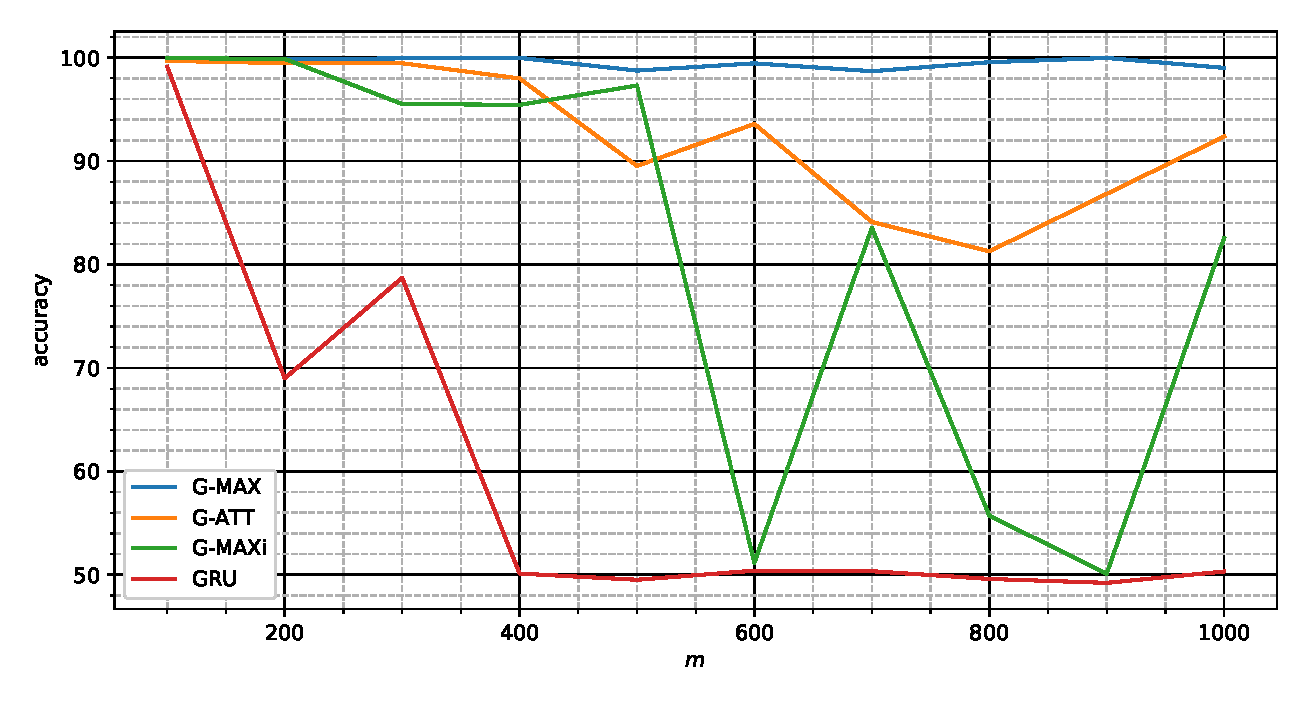
\includegraphics[width=\floatwidth]{imgMax/maxBaseDiff.eps}
  \caption{Max reached accuracy of model with max, attention, and base \ac{gru} on $\mathcal{D}^{(m)}$ for different dimensions of $m$.}
  \label{fig:testAccDiff}
\end{figure}
In \cref{fig:testAccDiff} we show the maximum reached accuracy for the
models, summarizing
\cref{fig:testAccBase,fig:testAccMax,fig:testAccInt} and adding the
model with the attention aggregator. The latter degrades faster than the
one with the max aggregation.

\subsection{Cancer register data}
Machine learning models need a training dataset in order to learn how
to perform predictions. A second test dataset — sampled from the same
distribution — is needed to assess the performances of the
classifier, and a third evaluation dataset is used to tune the
hyperparameters and to stop the training before the model overfits to
the training dataset. We decided to arrange our experiments on cancer
data in 
a setting that simulate a predictive task. We sorted the medical
records by insertion date, then we used the most recent $80\%$ of
records as test 
dataset, an equal amount of the remaining most recent records as
validation dataset, and the rest as training dataset. At the end the
training, validation, and test datasets have respectively $51\,101$,
$17\,034$, and $17\,035$ records.

We used the text in the $1.5$ millions unlabeled records, plus the
text in training datasets to train \ac{glove} word
vectors representations. We trained two different \ac{max} models, one
in an interpretable configuration that we call \ac{maxi} and one not
interpretable with 
best configuration that we call \ac{max}. We found the hyperparameters
configuration with grid search. 
\ac{maxi} have one \ac{gru} layer of dimension $256$
for \eqref{eq:maxModelRL} and \eqref{eq:maxModelRR}, 1 layer of
output dimension $68$ with aggregating function \eqref{eq:aggregation}
for \eqref{eq:maxModelF}, and zero layers for \eqref{eq:maxModelC}. 
\ac{max} have
one \ac{gru} layer with
dimension $128$ for \eqref{eq:maxModelRL} and \eqref{eq:maxModelRR},
one \ac{mlp} layer of dimension $512$ with aggregating function
\eqref{eq:aggregation} for \eqref{eq:maxModelF}, and
one layer of output dimension $68$ for \eqref{eq:maxModelC}.

We trained the models minimizing categorical cross entropy with Adam
\cite{kingma2014adam} using a learning rate of $0.001$. The
experiments were performed in \emph{PyTorch} on machines with
\emph{GeForce RTX 2080 Ti} 
GPU using batches of $32$ samples.

We compared \ac{max} and \ac{maxi} with a baseline of two stacked
bidirectional 
\ac{gru} layer of dimension $256$ and with \ac{bert} pretrained on the
same data where \ac{glove} where trained for the other models, and
fine-tuned on the training set.

\begin{table}
  \centering
  \caption{Results on cancer data}
  \label{tab:results}
  \begin{tabular}{|c|c|c|c|c|c|}
    \hline
    &Acc.&Acc. T3&Acc. T5&MAP&K\\
    \hline
    \hline
    \textbf{Site}&&&&&\\
    base&0.8977&0.9636&0.9764&0.9331&0.8848\\
    \acs{bert}&0.8980&0.9623&0.9768&0.9330&0.8852\\
    \acs{maxi}&0.8792&0.9533&0.9610&0.9190&0.8637\\
    \acs{maxh}&0.8980&0.9611&0.9773&0.9329&0.8851\\
    \acs{softmaxh}&0.8983&0.9617&0.9760&0.9329&0.8855\\
    \acs{softmax}&0.9008&0.9607&0.9749&0.9341&0.8883\\
    \acs{max}&\textbf{0.9024}&\textbf{0.9658}&\textbf{0.9797}&\textbf{0.9369}&\textbf{0.8901}\\
    \hline
    \hline
    \textbf{Morpho.}&&&&&\\
    base&0.8266&0.9402&0.9602&0.8881&0.8064\\
    \acs{bert}&0.8367&0.9267&0.9439&0.8870&0.8178\\
    \acs{maxi}&0.7317&0.9012&0.9305&0.8169&0.6964\\
    \acs{maxh}&0.8313&0.9382&0.9582&0.8894&0.8117\\
    \acs{softmaxh}&&&&&\\
    \acs{softmax}&\textbf{0.8424}&0.9445&0.9632&\textbf{0.8973}&\textbf{0.8240}\\
    \acs{max}&0.8394&\textbf{0.9452}&\textbf{0.9634}&0.8962&0.8207\\
    \hline
  \end{tabular}
\end{table}
In \cref{tab:results} we resumed the results of the models on the test
dataset. We report accuracy, \ac{map} and Cohen's kappa score (K).
\ac{map} is used in information
retrieval \cite{manning_introduction_2008}. It expresses how well the
correct class of a sample can be retrieved in 
the first results of the classifier output.
Cohen's kappa score is usually used to assess
the agreement of two annotators \cite{cohen_coefficient_1960}. It
measures the difference between the observed agreement and the
agreement that can happen choosing randomly the class. Can be used to
mitigate the bias caused by the unbalanced data set.

\begin{table}
  \centering
  \ttfamily
  \scriptsize
  \caption{Visualization of interpretable outputs.}
  \label{tab:multiAttention1}
  \begin{tabular}{|c|c|c|}
    \hline
    $y_i$&\textrm{Relevant} $\vect{h}_{i,j}$&$x_{i,j}$\textrm{, relevant} $\vect{h}_{i,j}$\\
    \hline
    61&\begin{minipage}{\attTableIcdoWidth}\att{61}{red}{100} \att{(PROSTATE}{red}{100} \att{GLAND)}{red}{100} \end{minipage}&\begin{minipage}{\attTableTextWidth}\att{DISOMOGENICITA}{red}{0} \att{'}{red}{0} \att{DIFFUSE}{red}{0} \att{.}{red}{0} \att{PSA}{red}{85} \att{NON}{red}{0} \att{PERVENUTO}{red}{0} \att{.}{red}{0} \att{ADENOCARCINOMA}{red}{0} \att{PROSTATICO}{red}{100} \att{A}{red}{0} \att{GRADO}{red}{1} \att{DI}{red}{0} \att{DIFFERENZIAZIONE}{red}{0} \att{MEDIO}{red}{0} \att{-}{red}{0} \att{BASSO}{red}{0} \att{(}{red}{0} \att{GLEASON}{red}{100} \att{3}{red}{4} \att{+}{red}{0} \att{4}{red}{0} \att{)}{red}{0} \att{NEI}{red}{0} \att{PRELIEVI}{red}{0} \att{DI}{red}{0} \att{CUI}{red}{0} \att{AI}{red}{0} \att{NN}{red}{0} \att{.}{red}{0} \att{2}{red}{0} \att{E}{red}{0} \att{3}{red}{0} \att{.}{red}{0} \att{AGOBIOPSIA}{red}{0} \att{DELLA}{red}{0} \att{PROSTATA}{red}{100} \att{:}{red}{0} \att{1}{red}{0} \att{)}{red}{0} \att{1}{red}{0} \att{PRELIEVO}{red}{0} \att{LL}{red}{0} \att{DX}{red}{0} \att{.}{red}{0} \att{2}{red}{0} \att{)}{red}{0} \att{2}{red}{0} \att{PRELIEVI}{red}{0} \att{ML}{red}{0} \att{DX}{red}{0} \att{.}{red}{0} \att{3}{red}{0} \att{)}{red}{0} \att{2}{red}{0} \att{PRELIEVI}{red}{0} \att{M}{red}{0} \att{DX}{red}{0} \att{.}{red}{0} \att{4}{red}{0} \att{)}{red}{0} \att{1}{red}{0} \att{PRELIEVO}{red}{0} \att{M}{red}{0} \att{SX}{red}{0} \att{.}{red}{0} \att{5}{red}{0} \att{)}{red}{0} \att{2}{red}{0} \att{PRELIEVI}{red}{0} \att{ML}{red}{0} \att{SX}{red}{0} \att{.}{red}{0} \att{6}{red}{0} \att{)}{red}{0} \att{1}{red}{0} \att{PRELIEVO}{red}{0} \att{LL}{red}{0} \att{SX}{red}{0} \att{.}{red}{0} \att{7}{red}{0} \att{)}{red}{0} \att{1}{red}{0} \att{PRELIEVO}{red}{0} \att{TRANSIZIONALE}{red}{54} \att{SX}{red}{1} \att{.}{red}{0} \att{8}{red}{0} \att{)}{red}{0} \att{1}{red}{0} \att{PRELIEVO}{red}{0} \att{TRANSIZIONALE}{red}{19} \att{DX}{red}{7} \att{.}{red}{0} \end{minipage}\\ % doc valid 49


    \hline
    20&\begin{minipage}{\attTableIcdoWidth}\att{\att{\att{18}{red}{100}}{green}{0}}{blue}{0} \att{\att{\att{(COLON)}{red}{100}}{green}{0}}{blue}{0} \\\\\att{\att{\att{20}{red}{0}}{green}{100}}{blue}{0} \att{\att{\att{(RECTUM)}{red}{0}}{green}{100}}{blue}{0} \\\\\att{\att{\att{21}{red}{0}}{green}{0}}{blue}{100} \att{\att{\att{(ANUS}{red}{0}}{green}{0}}{blue}{100} \att{\att{\att{AND}{red}{0}}{green}{0}}{blue}{100} \att{\att{\att{ANAL}{red}{0}}{green}{0}}{blue}{100} \att{\att{\att{CANAL)}{red}{0}}{green}{0}}{blue}{100} \end{minipage}&\begin{minipage}{\attTableTextWidth}\att{\att{\att{ISOLATI}{red}{0}}{green}{0}}{blue}{0} \att{\att{\att{FRAMMENTI}{red}{0}}{green}{0}}{blue}{0} \att{\att{\att{RIFERIBILI}{red}{0}}{green}{0}}{blue}{0} \att{\att{\att{AD}{red}{0}}{green}{0}}{blue}{0} \att{\att{\att{ADENOMA}{red}{0}}{green}{0}}{blue}{0} \att{\att{\att{TUBULARE}{red}{100}}{green}{0}}{blue}{0} \att{\att{\att{INTESTINALE}{red}{100}}{green}{1}}{blue}{0} \att{\att{\att{DI}{red}{2}}{green}{0}}{blue}{0} \att{\att{\att{ALTO}{red}{4}}{green}{0}}{blue}{0} \att{\att{\att{GRADO}{red}{1}}{green}{0}}{blue}{0} \att{\att{\att{.}{red}{0}}{green}{0}}{blue}{0} \att{\att{\att{FRAMMENTI}{red}{0}}{green}{0}}{blue}{0} \att{\att{\att{(}{red}{0}}{green}{0}}{blue}{0} \att{\att{\att{NR}{red}{0}}{green}{0}}{blue}{0} \att{\att{\att{.}{red}{0}}{green}{0}}{blue}{0} \att{\att{\att{2}{red}{0}}{green}{0}}{blue}{0} \att{\att{\att{)}{red}{0}}{green}{0}}{blue}{0} \att{\att{\att{DI}{red}{0}}{green}{0}}{blue}{0} \att{\att{\att{POLIPO}{red}{88}}{green}{63}}{blue}{0} \att{\att{\att{PEDUNCOLATO}{red}{100}}{green}{0}}{blue}{0} \att{\att{\att{A}{red}{0}}{green}{0}}{blue}{0} \att{\att{\att{20}{red}{0}}{green}{0}}{blue}{0} \att{\att{\att{CM}{red}{0}}{green}{0}}{blue}{0} \att{\att{\att{DALL}{red}{61}}{green}{0}}{blue}{0} \att{\att{\att{'}{red}{0}}{green}{0}}{blue}{0} \att{\att{\att{ORIFIZIO}{red}{0}}{green}{96}}{blue}{89} \att{\att{\att{ANALE}{red}{0}}{green}{100}}{blue}{100} \att{\att{\att{.}{red}{0}}{green}{30}}{blue}{0} \att{\att{\att{(}{red}{0}}{green}{0}}{blue}{0} \att{\att{\att{ESEGUITA}{red}{0}}{green}{0}}{blue}{0} \att{\att{\att{COLORAZIONE}{red}{0}}{green}{0}}{blue}{0} \att{\att{\att{EMATOSSILINA}{red}{0}}{green}{0}}{blue}{0} \att{\att{\att{-}{red}{0}}{green}{0}}{blue}{0} \att{\att{\att{EOSINA}{red}{0}}{green}{0}}{blue}{0} \att{\att{\att{)}{red}{0}}{green}{0}}{blue}{0} \att{\att{\att{.}{red}{0}}{green}{0}}{blue}{0} \end{minipage}\\ % doc valid 2


    \hline
    %61&\begin{minipage}{\attTableIcdoWidth}\att{61}{red}{100} \att{(PROSTATE}{red}{100} \att{GLAND)}{red}{100} \end{minipage}&\begin{minipage}{\attTableTextWidth}\att{DISOMOGENICITA}{red}{0} \att{'}{red}{0} \att{DIFFUSE}{red}{0} \att{.}{red}{0} \att{PSA}{red}{85} \att{NON}{red}{0} \att{PERVENUTO}{red}{0} \att{.}{red}{0} \att{ADENOCARCINOMA}{red}{0} \att{PROSTATICO}{red}{100} \att{A}{red}{0} \att{GRADO}{red}{1} \att{DI}{red}{0} \att{DIFFERENZIAZIONE}{red}{0} \att{MEDIO}{red}{0} \att{-}{red}{0} \att{BASSO}{red}{0} \att{(}{red}{0} \att{GLEASON}{red}{100} \att{3}{red}{4} \att{+}{red}{0} \att{4}{red}{0} \att{)}{red}{0} \att{NEI}{red}{0} \att{PRELIEVI}{red}{0} \att{DI}{red}{0} \att{CUI}{red}{0} \att{AI}{red}{0} \att{NN}{red}{0} \att{.}{red}{0} \att{2}{red}{0} \att{E}{red}{0} \att{3}{red}{0} \att{.}{red}{0} \att{AGOBIOPSIA}{red}{0} \att{DELLA}{red}{0} \att{PROSTATA}{red}{100} \att{:}{red}{0} \att{1}{red}{0} \att{)}{red}{0} \att{1}{red}{0} \att{PRELIEVO}{red}{0} \att{LL}{red}{0} \att{DX}{red}{0} \att{.}{red}{0} \att{2}{red}{0} \att{)}{red}{0} \att{2}{red}{0} \att{PRELIEVI}{red}{0} \att{ML}{red}{0} \att{DX}{red}{0} \att{.}{red}{0} \att{3}{red}{0} \att{)}{red}{0} \att{2}{red}{0} \att{PRELIEVI}{red}{0} \att{M}{red}{0} \att{DX}{red}{0} \att{.}{red}{0} \att{4}{red}{0} \att{)}{red}{0} \att{1}{red}{0} \att{PRELIEVO}{red}{0} \att{M}{red}{0} \att{SX}{red}{0} \att{.}{red}{0} \att{5}{red}{0} \att{)}{red}{0} \att{2}{red}{0} \att{PRELIEVI}{red}{0} \att{ML}{red}{0} \att{SX}{red}{0} \att{.}{red}{0} \att{6}{red}{0} \att{)}{red}{0} \att{1}{red}{0} \att{PRELIEVO}{red}{0} \att{LL}{red}{0} \att{SX}{red}{0} \att{.}{red}{0} \att{7}{red}{0} \att{)}{red}{0} \att{1}{red}{0} \att{PRELIEVO}{red}{0} \att{TRANSIZIONALE}{red}{54} \att{SX}{red}{1} \att{.}{red}{0} \att{8}{red}{0} \att{)}{red}{0} \att{1}{red}{0} \att{PRELIEVO}{red}{0} \att{TRANSIZIONALE}{red}{19} \att{DX}{red}{7} \att{.}{red}{0} \end{minipage}\\ % doc valid 49


    %\hline
    34&\begin{minipage}{\attTableIcdoWidth}\att{\att{\att{\att{34}{red}{100}}{green}{0}}{blue}{0}}{black}{0} \att{\att{\att{\att{(BRONCHUS}{red}{100}}{green}{0}}{blue}{0}}{black}{0} \att{\att{\att{\att{AND}{red}{100}}{green}{0}}{blue}{0}}{black}{0} \att{\att{\att{\att{LUNG)}{red}{100}}{green}{0}}{blue}{0}}{black}{0} \\\\\att{\att{\att{\att{56}{red}{0}}{green}{100}}{blue}{0}}{black}{0} \att{\att{\att{\att{(OVARY)}{red}{0}}{green}{100}}{blue}{0}}{black}{0} \\\\\att{\att{\att{\att{67}{red}{0}}{green}{0}}{blue}{100}}{black}{0} \att{\att{\att{\att{(BLADDER)}{red}{0}}{green}{0}}{blue}{100}}{black}{0} \\\\\att{\att{\att{\att{80}{red}{0}}{green}{0}}{blue}{0}}{black}{100} \att{\att{\att{\att{(UNKNOWN}{red}{0}}{green}{0}}{blue}{0}}{black}{100} \att{\att{\att{\att{PRIMARY}{red}{0}}{green}{0}}{blue}{0}}{black}{100} \att{\att{\att{\att{SITE)}{red}{0}}{green}{0}}{blue}{0}}{black}{100} \end{minipage}&\begin{minipage}{\attTableTextWidth}\att{\att{\att{\att{VERSAMENTO}{red}{5}}{green}{0}}{blue}{0}}{black}{0} \att{\att{\att{\att{PLEURICO}{red}{100}}{green}{55}}{blue}{0}}{black}{5} \att{\att{\att{\att{SX}{red}{24}}{green}{0}}{blue}{0}}{black}{0} \att{\att{\att{\att{DI}{red}{0}}{green}{0}}{blue}{0}}{black}{0} \att{\att{\att{\att{N}{red}{0}}{green}{0}}{blue}{0}}{black}{0} \att{\att{\att{\att{.}{red}{0}}{green}{0}}{blue}{0}}{black}{0} \att{\att{\att{\att{D}{red}{0}}{green}{0}}{blue}{0}}{black}{0} \att{\att{\att{\att{.}{red}{0}}{green}{0}}{blue}{0}}{black}{0} \att{\att{\att{\att{D}{red}{0}}{green}{0}}{blue}{0}}{black}{0} \att{\att{\att{\att{.}{red}{0}}{green}{0}}{blue}{0}}{black}{0} \att{\att{\att{\att{E}{red}{0}}{green}{0}}{blue}{0}}{black}{0} \att{\att{\att{\att{ADDENSAMENTI}{red}{16}}{green}{0}}{blue}{0}}{black}{0} \att{\att{\att{\att{POLMONARI}{red}{100}}{green}{0}}{blue}{0}}{black}{0} \att{\att{\att{\att{DI}{red}{0}}{green}{0}}{blue}{0}}{black}{0} \att{\att{\att{\att{N}{red}{0}}{green}{0}}{blue}{0}}{black}{0} \att{\att{\att{\att{.}{red}{0}}{green}{0}}{blue}{0}}{black}{0} \att{\att{\att{\att{D}{red}{0}}{green}{0}}{blue}{0}}{black}{0} \att{\att{\att{\att{.}{red}{0}}{green}{0}}{blue}{0}}{black}{0} \att{\att{\att{\att{D}{red}{0}}{green}{0}}{blue}{0}}{black}{0} \att{\att{\att{\att{.}{red}{0}}{green}{0}}{blue}{0}}{black}{0} \att{\att{\att{\att{,}{red}{0}}{green}{0}}{blue}{0}}{black}{0} \att{\att{\att{\att{NODULI}{red}{0}}{green}{0}}{blue}{0}}{black}{0} \att{\att{\att{\att{PARETE}{red}{0}}{green}{0}}{blue}{28}}{black}{0} \att{\att{\att{\att{ADDOMINALE}{red}{1}}{green}{0}}{blue}{0}}{black}{0} \att{\att{\att{\att{.}{red}{0}}{green}{0}}{blue}{0}}{black}{0} \att{\att{\att{\att{INFILTRAZIONE}{red}{0}}{green}{0}}{blue}{0}}{black}{0} \att{\att{\att{\att{CANCERIGNA}{red}{100}}{green}{0}}{blue}{0}}{black}{13} \att{\att{\att{\att{DEGLI}{red}{100}}{green}{0}}{blue}{0}}{black}{83} \att{\att{\att{\att{STROMI}{red}{7}}{green}{0}}{blue}{0}}{black}{100} \att{\att{\att{\att{CONNETTIVO}{red}{0}}{green}{0}}{blue}{0}}{black}{0} \att{\att{\att{\att{-}{red}{1}}{green}{0}}{blue}{0}}{black}{0} \att{\att{\att{\att{ADIPOSI}{red}{0}}{green}{0}}{blue}{0}}{black}{78} \att{\att{\att{\att{.}{red}{30}}{green}{0}}{blue}{0}}{black}{1} \att{\att{\att{\att{IMMUNOISTOCHIMICA}{red}{100}}{green}{0}}{blue}{0}}{black}{95} \att{\att{\att{\att{:}{red}{17}}{green}{0}}{blue}{0}}{black}{98} \att{\att{\att{\att{CK7}{red}{100}}{green}{0}}{blue}{0}}{black}{100} \att{\att{\att{\att{+}{red}{99}}{green}{0}}{blue}{0}}{black}{0} \att{\att{\att{\att{,}{red}{77}}{green}{0}}{blue}{0}}{black}{51} \att{\att{\att{\att{CK20}{red}{100}}{green}{0}}{blue}{0}}{black}{100} \att{\att{\att{\att{-}{red}{100}}{green}{0}}{blue}{0}}{black}{1} \att{\att{\att{\att{,}{red}{84}}{green}{0}}{blue}{0}}{black}{37} \att{\att{\att{\att{TTF}{red}{100}}{green}{0}}{blue}{0}}{black}{100} \att{\att{\att{\att{-}{red}{100}}{green}{0}}{blue}{0}}{black}{0} \att{\att{\att{\att{1}{red}{3}}{green}{0}}{blue}{0}}{black}{0} \att{\att{\att{\att{-}{red}{31}}{green}{0}}{blue}{0}}{black}{0} \att{\att{\att{\att{,}{red}{69}}{green}{0}}{blue}{0}}{black}{0} \att{\att{\att{\att{PROTEINA}{red}{99}}{green}{0}}{blue}{0}}{black}{70} \att{\att{\att{\att{S}{red}{0}}{green}{0}}{blue}{0}}{black}{4} \att{\att{\att{\att{-}{red}{0}}{green}{0}}{blue}{0}}{black}{0} \att{\att{\att{\att{100}{red}{2}}{green}{0}}{blue}{0}}{black}{1} \att{\att{\att{\att{-}{red}{0}}{green}{0}}{blue}{0}}{black}{0} \att{\att{\att{\att{.}{red}{0}}{green}{0}}{blue}{0}}{black}{0} \att{\att{\att{\att{LESIONE}{red}{0}}{green}{0}}{blue}{0}}{black}{0} \att{\att{\att{\att{DI}{red}{0}}{green}{0}}{blue}{0}}{black}{0} \att{\att{\att{\att{CM}{red}{0}}{green}{0}}{blue}{0}}{black}{0} \att{\att{\att{\att{2}{red}{1}}{green}{0}}{blue}{0}}{black}{0} \att{\att{\att{\att{,}{red}{0}}{green}{0}}{blue}{0}}{black}{0} \att{\att{\att{\att{0}{red}{28}}{green}{0}}{blue}{0}}{black}{0} \att{\att{\att{\att{X}{red}{0}}{green}{0}}{blue}{0}}{black}{0} \att{\att{\att{\att{1}{red}{0}}{green}{0}}{blue}{0}}{black}{0} \att{\att{\att{\att{,}{red}{1}}{green}{0}}{blue}{0}}{black}{0} \att{\att{\att{\att{3}{red}{0}}{green}{0}}{blue}{0}}{black}{0} \att{\att{\att{\att{X}{red}{0}}{green}{0}}{blue}{0}}{black}{0} \att{\att{\att{\att{0}{red}{2}}{green}{0}}{blue}{0}}{black}{0} \att{\att{\att{\att{,}{red}{7}}{green}{0}}{blue}{0}}{black}{0} \att{\att{\att{\att{7}{red}{0}}{green}{0}}{blue}{0}}{black}{0} \att{\att{\att{\att{.}{red}{0}}{green}{0}}{blue}{0}}{black}{0} \att{\att{\att{\att{1}{red}{3}}{green}{0}}{blue}{0}}{black}{0} \att{\att{\att{\att{-}{red}{3}}{green}{0}}{blue}{0}}{black}{0} \att{\att{\att{\att{2}{red}{0}}{green}{0}}{blue}{0}}{black}{0} \att{\att{\att{\att{)}{red}{0}}{green}{0}}{blue}{0}}{black}{0} \att{\att{\att{\att{SEZIONI}{red}{23}}{green}{0}}{blue}{0}}{black}{0} \att{\att{\att{\att{SERIATE}{red}{87}}{green}{0}}{blue}{0}}{black}{3} \att{\att{\att{\att{.}{red}{65}}{green}{0}}{blue}{0}}{black}{0} \end{minipage}\\ % doc valid 923


    \hline
  \end{tabular}
\end{table}
The interpretable model is not powerful as \ac{max}, and in this task
is not even as the baseline, but it can be used as a
classification support and to 
gain insight in the classification process. In
\cref{tab:multiAttention1} we show three different samples where we
underline with different colors --- only for the indicated relevant
codes --- the values of $\vect{h}_{i,j}$ in \eqref{eq:maxModelF}. We
consider a code relevant if the corresponding value in the
68-dimension vector $\vect{h}_{i,j}$ is greater than $0.1$. In the
first sample, that was correctly classified, all the terms related to
prostate gland cancer are strongly underlined. Apart from
\emph{prostatico} and \emph{prostata} that are Italian terms for
\emph{prostatic} and \emph{prostate}, the main underlined terms are
\emph{PSA} (Prostate-Specific Antigene) and \emph{Gleason} score that
are two common exams in prostate cancer cases
\cite{brimo2013prostate}.

The second sample is a more difficult
document, it is roughly translated in english:\\
%\smallskip\noindent
\begin{small}
  \ttfamily
  \begin{tabular}{l}
    ISOLATED FRAGMENTS ATTRIBUTABLES\\
    TO HIGH DEGREE\\
    INTESTINAL TUBULAR ADENOMA.\\
    FRAGMENTS (NR. 2) OF PEDUNCULATED\\
    POLYPUS AT 20 CM FROM\\
    THE ANAL ORIFICE. (PERFORMED\\
    HEMATOXYLIN-EOSIN COLORING).
\end{tabular}
\end{small}\\
For this sample, the model propose the three classification codes \emph{18},
\emph{20}, and \emph{21} (with value $1$ for both \emph{18} and
\emph{20}, and little less for \emph{21}). It suggests that the terms
\emph{intestinal tubular adenoma} and \emph{pedunculated polypus} are
related to colon, \emph{polypus} can be related also to rectum, and
\emph{anal orifice} is related to rectum and anus. Note that this
record was labeled with the code for rectum, while the medical report
explicitly mention that the fragments have been extracted at 20 cm
from the anal orifice (the human rectum is long approximately 12 cm
and the anal canal 3-5 cm \cite{greene2006ajcc}).

The third sample is an even more complex record, in english is
translated:\\
\begin{small}
  \ttfamily
  \begin{tabular}{l}
    LEFT PLEURAL EFFUSION OF\\
    UNKNOWN ORIGIN AND LUNG\\
    THICKENING OF UNKNOWN ORIGIN,\\
    NODULES OF THE ABDOMINAL WALL.\\
    CANCEROUS INFILTRATION OF THE\\
    CONNECTIVE-ADIPOSE STROMA.\\
    IMMUNOHISTOCHEMICAL: CK7 +,\\
    CK20 -, TTF-1 -, PROTEIN\\
    S-100 -. 2 CM LESION,\\
    0 X 1,3 X 0,7. 1-2)\\
    SERIAL SECTIONS.
\end{tabular}
\end{small}\\
The model classifies the record mainly with codes \emph{34} and
\emph{80}, and less with \emph{56} and \emph{67}. It underlines with
the lung code the terms
\emph{plurial effusion} and \emph{lung thickening}, but is interesting
that it also underlines the immunohistochemical results. The
positive \emph{CK7}, negative \emph{CK20} pattern represents a common
diagnosis 
of lung origin for metastatic adenocarcinoma
\cite{kummar2002cytokeratin}. Also immunohistochemistry is a common
approach in the diagnosis of tumors of uncertain origin
\cite{duraiyan2012applications}. This can be the reason for the
underlying with code \emph{80} of the immunoistochemical part.
It is interesting to note also that \emph{pleuric} is
suggested to be related to ovary cancer, in fact the pleural cavity
constitutes the most frequently extra abdominal metastatic site in
ovarian carcinoma \cite{porcel2012pleural}.

\begin{figure}
  \centering
  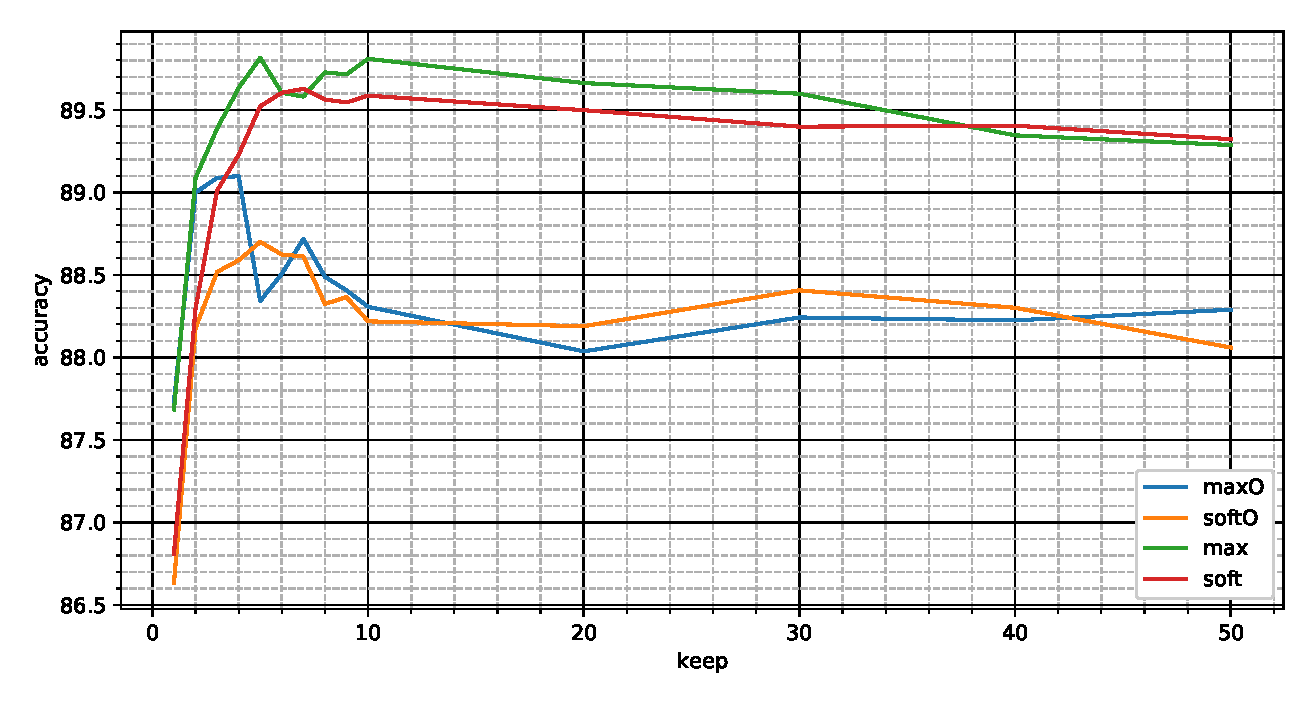
\includegraphics[width=\floatwidth]{img/plotSintex.eps}
  \caption{.}
  \label{fig:sintex}
\end{figure}
To quantify the effectiveness of the interpretability, we designed an
experiment where the dataset is created taking for each document the
first $k$ words selected by  
ordering the results of the aggregator, $u_t$ in case of max,
$a_t(\vect{u};\theta^a)u_t$ in case of attention. In \cref{fig:sintex}
we plot the accuracy obtained training a plain \ac{gru} model on the
cleaned datasets, increasing $k$. 



%%% Local Variables:
%%% mode: latex
%%% TeX-master: "thesis"
%%% End:

% \include{.. add your chapters}
% \chapter{Conclusions}
Since the cancer registration process is partially based on manual
revision, including also the interpretation of the free text in
pathological reports, significant delays in data production and
publication may occur. This weakens data relevance for the purpose of
assessing compliance with updated regional recommended integrated case
pathways, as well as for public health purposes. Improving automated
methods to generate a list of putative incident cases and to
automatically estimate process indicators is thus an opportunity to
perform an up-to-date evaluation of cancer-care quality. In
particular, machine learning techniques like the ones presented in
this paper could overcome the delay in cancer case definition by the
cancer registry and allow a powerful tool for timely indicators
computation. The implementation of this procedure could guarantee an
automated and validated instrument to monitor and evaluate diagnostic
and therapeutic pathways.

We analyzed the available data and created different models in order
to implement an automated classification system. We obtained very
encouraging results in classifying cancer cases based on the
interpretation of free text in the data-flow of pathology
reports. This suggests that machine learning methods can be usefully
leveraged in this context. Moreover, we demonstrated that unlabeled
data can 
be effectively used to construct useful word vectors and improve
classification accuracy. 

Our models also have the added value that they can be
utilized to retrieve records adjusting the precision-recall trade-off.

The use of administrative data sources that are up to date combined
with powerful machine learning techniques to automate text
classification is in the interest of the development of a standardized
surveillance system at Regional and National level. Stakeholders and
decision makers need timely and updated indicators to evaluate and
plan healthcare activities. The availability of timely indicators,
routinely and automatically produced, is technically possible. The
main novelty of this work is to show the power of machine learning
techniques applied to the classification of free text pathological
records. This was not yet been systematically implemented in other
Italian cancer registries. This provides a useful monitor tool for
cancer patients pathways, allowing to describe population’s general
health state and to establish public health goals.

The results of the interpretable models can be used to
assist the human classification process on simple records. It can be
used as
a form of text compression, highlighting the most important terms. On
more complex records it can be used to leverage the knowledge of the
model to gain insight on the decision process. To overcome the
limitations of the interpretable
model respect to the general model, in terms of
classification metrics, is it possible to combine the two variants. The
general model can be used to give a more
authoritative classification on the samples while at the same time,
the interpretable model can highlight the same samples.

We compared novel deep learning techniques and more classical models
to pathology records. In this specific context we did not obtain
significant improvements using novel deep learning approaches respect
to classic machine learning methods. Also, the attention methods
usually employed in text classification tasks do not have better
results respect to a more simple max pooling hard attention. Furthermore,
hierarchical models do not work better than plain models. Unsupervised
methods, in particular Word Vectors,
can be used successfully in the
domain of pathological text records. At the best of our knowledge, this
is the first large scale study of deep learning methods applied to
pathology records. Other studies where performed on smaller datasets
with records labeled with less classes.

Regarding the questions in \cref{sec:motivation}, Q1 is answered by
the fact that we implemented several different models to a large scale
dataset of cancer pathology reports. Q2 is answered by the fact that
we used attention models and \ac{bert} in our experiments. To answer
to Q3, from our experiments we have evidence that by using deep learning
methods we do not have a breakthrough compared to classic
\ac{ml} approaches in this specific domain. Regarding Q4, we observe
that hierarchical models are not beneficial in this context. Moreover,
we achieve a little improvement by using attention models, but in
this context a simple max aggregation is equally powerful to the
commonly used attention. About Q5 we observe a successful improvement
when we leverage the unlabeled data, thus we can conclude that
unsupervised techniques can be successfully used in this
context. Finally, in relation to Q6 we studied the potentialities of
interpretable models in the pathology records context.

%%% Local Variables:
%%% mode: latex
%%% TeX-master: "thesis"
%%% End:

\appendix{
%  \chapter{Details of experiments}
\label{app:details}

Totally optional
\section{Setup of Experiment 1}
\section{Detailed results}
  % Optional, for details that cannot fit the main body
  \chapter{Publications}
\label{app:publications}

\subsection*{Journal papers}
\begin{enumerate}
\item \textbf{Stefano Martina}, Leonardo Ventura, Paolo Frasconi,
  ``Classification of cancer pathology reports: a large-scale comparative study'', \textit{Journal of Biomedical and Health Informatics}, in
  review.
  \textbf{Candidate's contributions}: prepared dataset, designed
  methods and experiments, designed algorithms
\end{enumerate}
\subsection*{Peer reviewed conference papers}
\subsection*{Workshop papers}
\subsection*{Papers under review}
\subsection*{Other}
(e.g. ArXiv preprints not yet submitted)


 % Mandatory
}
% End EDIT
%%%%%%%%%%%%%%%%%%%%%%%%%%%%%%%%%%%%%%%%%%%%%%%%%%%%%%%%%%%%%%%%%%%%%%%%%%%%%
\bibliographystyle{apalike}
\bibliography{Oncology,more}
\end{document}

%%% Local Variables:
%%% mode: latex
%%% TeX-master: t
%%% End:
